\documentclass[twoside]{book}

% Packages required by doxygen
\usepackage{fixltx2e}
\usepackage{calc}
\usepackage{doxygen}
\usepackage[export]{adjustbox} % also loads graphicx
\usepackage{graphicx}
\usepackage[utf8]{inputenc}
\usepackage{makeidx}
\usepackage{multicol}
\usepackage{multirow}
\PassOptionsToPackage{warn}{textcomp}
\usepackage{textcomp}
\usepackage[nointegrals]{wasysym}
\usepackage[table]{xcolor}

% Font selection
\usepackage[T1]{fontenc}
\usepackage[scaled=.90]{helvet}
\usepackage{courier}
\usepackage{amssymb}
\usepackage{sectsty}
\renewcommand{\familydefault}{\sfdefault}
\allsectionsfont{%
  \fontseries{bc}\selectfont%
  \color{darkgray}%
}
\renewcommand{\DoxyLabelFont}{%
  \fontseries{bc}\selectfont%
  \color{darkgray}%
}
\newcommand{\+}{\discretionary{\mbox{\scriptsize$\hookleftarrow$}}{}{}}

% Page & text layout
\usepackage{geometry}
\geometry{%
  a4paper,%
  top=2.5cm,%
  bottom=2.5cm,%
  left=2.5cm,%
  right=2.5cm%
}
\tolerance=750
\hfuzz=15pt
\hbadness=750
\setlength{\emergencystretch}{15pt}
\setlength{\parindent}{0cm}
\setlength{\parskip}{3ex plus 2ex minus 2ex}
\makeatletter
\renewcommand{\paragraph}{%
  \@startsection{paragraph}{4}{0ex}{-1.0ex}{1.0ex}{%
    \normalfont\normalsize\bfseries\SS@parafont%
  }%
}
\renewcommand{\subparagraph}{%
  \@startsection{subparagraph}{5}{0ex}{-1.0ex}{1.0ex}{%
    \normalfont\normalsize\bfseries\SS@subparafont%
  }%
}
\makeatother

% Headers & footers
\usepackage{fancyhdr}
\pagestyle{fancyplain}
\fancyhead[LE]{\fancyplain{}{\bfseries\thepage}}
\fancyhead[CE]{\fancyplain{}{}}
\fancyhead[RE]{\fancyplain{}{\bfseries\leftmark}}
\fancyhead[LO]{\fancyplain{}{\bfseries\rightmark}}
\fancyhead[CO]{\fancyplain{}{}}
\fancyhead[RO]{\fancyplain{}{\bfseries\thepage}}
\fancyfoot[LE]{\fancyplain{}{}}
\fancyfoot[CE]{\fancyplain{}{}}
\fancyfoot[RE]{\fancyplain{}{\bfseries\scriptsize Generated by Doxygen }}
\fancyfoot[LO]{\fancyplain{}{\bfseries\scriptsize Generated by Doxygen }}
\fancyfoot[CO]{\fancyplain{}{}}
\fancyfoot[RO]{\fancyplain{}{}}
\renewcommand{\footrulewidth}{0.4pt}
\renewcommand{\chaptermark}[1]{%
  \markboth{#1}{}%
}
\renewcommand{\sectionmark}[1]{%
  \markright{\thesection\ #1}%
}

% Indices & bibliography
\usepackage{natbib}
\usepackage[titles]{tocloft}
\setcounter{tocdepth}{3}
\setcounter{secnumdepth}{5}
\makeindex

% Hyperlinks (required, but should be loaded last)
\usepackage{ifpdf}
\ifpdf
  \usepackage[pdftex,pagebackref=true]{hyperref}
\else
  \usepackage[ps2pdf,pagebackref=true]{hyperref}
\fi
\hypersetup{%
  colorlinks=true,%
  linkcolor=blue,%
  citecolor=blue,%
  unicode%
}

% Custom commands
\newcommand{\clearemptydoublepage}{%
  \newpage{\pagestyle{empty}\cleardoublepage}%
}

\usepackage{caption}
\captionsetup{labelsep=space,justification=centering,font={bf},singlelinecheck=off,skip=4pt,position=top}

%===== C O N T E N T S =====

\begin{document}

% Titlepage & ToC
\hypersetup{pageanchor=false,
             bookmarksnumbered=true,
             pdfencoding=unicode
            }
\pagenumbering{alph}
\begin{titlepage}
\vspace*{7cm}
\begin{center}%
{\Large The Resume Shotgun }\\
\vspace*{1cm}
{\large Generated by Doxygen 1.8.13}\\
\end{center}
\end{titlepage}
\clearemptydoublepage
\pagenumbering{roman}
\tableofcontents
\clearemptydoublepage
\pagenumbering{arabic}
\hypersetup{pageanchor=true}

%--- Begin generated contents ---
\chapter{Application\+\_\+3\+X\+A3\+\_\+\+L01\+\_\+\+G\+R\+P05 Source Code}
\label{md__home_gab_repos_application_3xa3_l01_grp05_src_README}
\Hypertarget{md__home_gab_repos_application_3xa3_l01_grp05_src_README}
The folders and files for this project are as follows\+: 
\chapter{Hierarchical Index}
\section{Class Hierarchy}
This inheritance list is sorted roughly, but not completely, alphabetically\+:\begin{DoxyCompactList}
\item \contentsline{section}{indeed.\+Indeed}{\pageref{classindeed_1_1Indeed}}{}
\item \contentsline{section}{Job.\+Job}{\pageref{classJob_1_1Job}}{}
\item \contentsline{section}{pdf\+Reader.\+pdf\+Reader}{\pageref{classpdfReader_1_1pdfReader}}{}
\item Test\+Case\begin{DoxyCompactList}
\item \contentsline{section}{test.\+indeed\+Test}{\pageref{classtest_1_1indeedTest}}{}
\item \contentsline{section}{test.\+template\+Test}{\pageref{classtest_1_1templateTest}}{}
\item \contentsline{section}{test.\+user\+Profile\+Base}{\pageref{classtest_1_1userProfileBase}}{}
\begin{DoxyCompactList}
\item \contentsline{section}{test.\+menu\+Test}{\pageref{classtest_1_1menuTest}}{}
\item \contentsline{section}{test.\+user\+Profile\+Test}{\pageref{classtest_1_1userProfileTest}}{}
\end{DoxyCompactList}
\end{DoxyCompactList}
\item \contentsline{section}{user\+Profile.\+user\+Profile}{\pageref{classuserProfile_1_1userProfile}}{}
\end{DoxyCompactList}

\chapter{Class Index}
\section{Class List}
Here are the classes, structs, unions and interfaces with brief descriptions\+:\begin{DoxyCompactList}
\item\contentsline{section}{\hyperlink{classpdfReader_1_1PDF}{pdf\+Reader.\+P\+DF} \\*This class represents a \hyperlink{classpdfReader_1_1PDF}{P\+DF} document }{\pageref{classpdfReader_1_1PDF}}{}
\item\contentsline{section}{\hyperlink{classtest_1_1templateTest}{test.\+template\+Test} \\*Tests }{\pageref{classtest_1_1templateTest}}{}
\item\contentsline{section}{\hyperlink{classuserProfile_1_1userProfile}{user\+Profile.\+user\+Profile} \\*This class represents the preferences of a user for job searching }{\pageref{classuserProfile_1_1userProfile}}{}
\item\contentsline{section}{\hyperlink{classtest_1_1userProfileBase}{test.\+user\+Profile\+Base} \\*Setup for user\+Profile module }{\pageref{classtest_1_1userProfileBase}}{}
\item\contentsline{section}{\hyperlink{classtest_1_1userProfileTest}{test.\+user\+Profile\+Test} \\*Tests for user\+Profile module }{\pageref{classtest_1_1userProfileTest}}{}
\end{DoxyCompactList}

\chapter{File Index}
\section{File List}
Here is a list of all documented files with brief descriptions\+:\begin{DoxyCompactList}
\item\contentsline{section}{/home/gab/repos/application\+\_\+3xa3\+\_\+l01\+\_\+grp05/src/\hyperlink{apply_8py}{apply.\+py} \\*Main module used for the application proccess }{\pageref{apply_8py}}{}
\item\contentsline{section}{/home/gab/repos/application\+\_\+3xa3\+\_\+l01\+\_\+grp05/src/\hyperlink{get__links__glassdoor_8py}{get\+\_\+links\+\_\+glassdoor.\+py} \\*Module used for collecting links from the Glassdoor site }{\pageref{get__links__glassdoor_8py}}{}
\item\contentsline{section}{/home/gab/repos/application\+\_\+3xa3\+\_\+l01\+\_\+grp05/src/\hyperlink{get__links__indeed_8py}{get\+\_\+links\+\_\+indeed.\+py} \\*Module that signs into Indeed website }{\pageref{get__links__indeed_8py}}{}
\item\contentsline{section}{/home/gab/repos/application\+\_\+3xa3\+\_\+l01\+\_\+grp05/src/\hyperlink{menu_8py}{menu.\+py} \\*Allows the user to easily view and set new values for a user profile }{\pageref{menu_8py}}{}
\item\contentsline{section}{/home/gab/repos/application\+\_\+3xa3\+\_\+l01\+\_\+grp05/src/\hyperlink{menuMessages_8py}{menu\+Messages.\+py} \\*Interface messages module }{\pageref{menuMessages_8py}}{}
\item\contentsline{section}{/home/gab/repos/application\+\_\+3xa3\+\_\+l01\+\_\+grp05/src/\hyperlink{pdfReader_8py}{pdf\+Reader.\+py} \\*P\+DF Interpretor }{\pageref{pdfReader_8py}}{}
\item\contentsline{section}{/home/gab/repos/application\+\_\+3xa3\+\_\+l01\+\_\+grp05/src/\hyperlink{sites_8py}{sites.\+py} \\*Sites \char`\"{}dictionary\char`\"{} }{\pageref{sites_8py}}{}
\item\contentsline{section}{/home/gab/repos/application\+\_\+3xa3\+\_\+l01\+\_\+grp05/src/\hyperlink{test_8py}{test.\+py} \\*Testing for modules }{\pageref{test_8py}}{}
\item\contentsline{section}{/home/gab/repos/application\+\_\+3xa3\+\_\+l01\+\_\+grp05/src/\hyperlink{userProfile_8py}{user\+Profile.\+py} \\*User profile module }{\pageref{userProfile_8py}}{}
\end{DoxyCompactList}

\chapter{Class Documentation}
\hypertarget{classpdfReader_1_1PDF}{}\section{pdf\+Reader.\+P\+DF Class Reference}
\label{classpdfReader_1_1PDF}\index{pdf\+Reader.\+P\+DF@{pdf\+Reader.\+P\+DF}}


This class represents a \hyperlink{classpdfReader_1_1PDF}{P\+DF} document.  


\subsection*{Public Member Functions}
\begin{DoxyCompactItemize}
\item 
def \hyperlink{classpdfReader_1_1PDF_ad3a030d731fe9fdbdd25cbdf2811cfd9}{\+\_\+\+\_\+init\+\_\+\+\_\+} (self, path)
\begin{DoxyCompactList}\small\item\em Constructor for \hyperlink{classpdfReader_1_1PDF}{P\+DF}. \end{DoxyCompactList}\item 
\mbox{\Hypertarget{classpdfReader_1_1PDF_a4fc2e001f7e9dc04f2a77b2f7988e7d9}\label{classpdfReader_1_1PDF_a4fc2e001f7e9dc04f2a77b2f7988e7d9}} 
def \hyperlink{classpdfReader_1_1PDF_a4fc2e001f7e9dc04f2a77b2f7988e7d9}{display} (self)
\begin{DoxyCompactList}\small\item\em Displays the document to the user in an interactive window. \end{DoxyCompactList}\item 
def \hyperlink{classpdfReader_1_1PDF_adecd6d310fcbaf65067825dcb000c6e5}{search} (self, key)
\begin{DoxyCompactList}\small\item\em Searches the \hyperlink{classpdfReader_1_1PDF}{P\+DF} for a specified keyword. \end{DoxyCompactList}\item 
def \hyperlink{classpdfReader_1_1PDF_ae0c66e62a60c32cf66340a7f63b37706}{split} (self, page)
\begin{DoxyCompactList}\small\item\em Splits the \hyperlink{classpdfReader_1_1PDF}{P\+DF} document into two seperate \hyperlink{classpdfReader_1_1PDF}{P\+DF} objects. \end{DoxyCompactList}\item 
def \hyperlink{classpdfReader_1_1PDF_a64f25f9ee8d33642377bcec567898a23}{merge} (self, pdf)
\begin{DoxyCompactList}\small\item\em Merges two \hyperlink{classpdfReader_1_1PDF}{P\+DF} objects into a single object. \end{DoxyCompactList}\end{DoxyCompactItemize}


\subsection{Detailed Description}
This class represents a \hyperlink{classpdfReader_1_1PDF}{P\+DF} document. 

Assumes all inputs are of the correct type 

\subsection{Constructor \& Destructor Documentation}
\mbox{\Hypertarget{classpdfReader_1_1PDF_ad3a030d731fe9fdbdd25cbdf2811cfd9}\label{classpdfReader_1_1PDF_ad3a030d731fe9fdbdd25cbdf2811cfd9}} 
\index{pdf\+Reader\+::\+P\+DF@{pdf\+Reader\+::\+P\+DF}!\+\_\+\+\_\+init\+\_\+\+\_\+@{\+\_\+\+\_\+init\+\_\+\+\_\+}}
\index{\+\_\+\+\_\+init\+\_\+\+\_\+@{\+\_\+\+\_\+init\+\_\+\+\_\+}!pdf\+Reader\+::\+P\+DF@{pdf\+Reader\+::\+P\+DF}}
\subsubsection{\texorpdfstring{\+\_\+\+\_\+init\+\_\+\+\_\+()}{\_\_init\_\_()}}
{\footnotesize\ttfamily def pdf\+Reader.\+P\+D\+F.\+\_\+\+\_\+init\+\_\+\+\_\+ (\begin{DoxyParamCaption}\item[{}]{self,  }\item[{}]{path }\end{DoxyParamCaption})}



Constructor for \hyperlink{classpdfReader_1_1PDF}{P\+DF}. 

Defines a \hyperlink{classpdfReader_1_1PDF}{P\+DF} based on a file path 
\begin{DoxyParams}{Parameters}
{\em path} & String value which describes the file path to the desired document \\
\hline
\end{DoxyParams}


\subsection{Member Function Documentation}
\mbox{\Hypertarget{classpdfReader_1_1PDF_a64f25f9ee8d33642377bcec567898a23}\label{classpdfReader_1_1PDF_a64f25f9ee8d33642377bcec567898a23}} 
\index{pdf\+Reader\+::\+P\+DF@{pdf\+Reader\+::\+P\+DF}!merge@{merge}}
\index{merge@{merge}!pdf\+Reader\+::\+P\+DF@{pdf\+Reader\+::\+P\+DF}}
\subsubsection{\texorpdfstring{merge()}{merge()}}
{\footnotesize\ttfamily def pdf\+Reader.\+P\+D\+F.\+merge (\begin{DoxyParamCaption}\item[{}]{self,  }\item[{}]{pdf }\end{DoxyParamCaption})}



Merges two \hyperlink{classpdfReader_1_1PDF}{P\+DF} objects into a single object. 


\begin{DoxyParams}{Parameters}
{\em pdf} & \hyperlink{classpdfReader_1_1PDF}{P\+DF} object that will be merged with current \hyperlink{classpdfReader_1_1PDF}{P\+DF} \\
\hline
\end{DoxyParams}
\begin{DoxyReturn}{Returns}
\hyperlink{classpdfReader_1_1PDF}{P\+DF} object 
\end{DoxyReturn}
\mbox{\Hypertarget{classpdfReader_1_1PDF_adecd6d310fcbaf65067825dcb000c6e5}\label{classpdfReader_1_1PDF_adecd6d310fcbaf65067825dcb000c6e5}} 
\index{pdf\+Reader\+::\+P\+DF@{pdf\+Reader\+::\+P\+DF}!search@{search}}
\index{search@{search}!pdf\+Reader\+::\+P\+DF@{pdf\+Reader\+::\+P\+DF}}
\subsubsection{\texorpdfstring{search()}{search()}}
{\footnotesize\ttfamily def pdf\+Reader.\+P\+D\+F.\+search (\begin{DoxyParamCaption}\item[{}]{self,  }\item[{}]{key }\end{DoxyParamCaption})}



Searches the \hyperlink{classpdfReader_1_1PDF}{P\+DF} for a specified keyword. 


\begin{DoxyParams}{Parameters}
{\em key} & String value which is searched for \\
\hline
\end{DoxyParams}
\begin{DoxyReturn}{Returns}
Boolean value based on whether or not the key could be found 
\end{DoxyReturn}
\mbox{\Hypertarget{classpdfReader_1_1PDF_ae0c66e62a60c32cf66340a7f63b37706}\label{classpdfReader_1_1PDF_ae0c66e62a60c32cf66340a7f63b37706}} 
\index{pdf\+Reader\+::\+P\+DF@{pdf\+Reader\+::\+P\+DF}!split@{split}}
\index{split@{split}!pdf\+Reader\+::\+P\+DF@{pdf\+Reader\+::\+P\+DF}}
\subsubsection{\texorpdfstring{split()}{split()}}
{\footnotesize\ttfamily def pdf\+Reader.\+P\+D\+F.\+split (\begin{DoxyParamCaption}\item[{}]{self,  }\item[{}]{page }\end{DoxyParamCaption})}



Splits the \hyperlink{classpdfReader_1_1PDF}{P\+DF} document into two seperate \hyperlink{classpdfReader_1_1PDF}{P\+DF} objects. 


\begin{DoxyParams}{Parameters}
{\em page} & Integer value defining at which page the \hyperlink{classpdfReader_1_1PDF}{P\+DF} should be split \\
\hline
\end{DoxyParams}
\begin{DoxyReturn}{Returns}
Tuple of \hyperlink{classpdfReader_1_1PDF}{P\+DF} objects 
\end{DoxyReturn}


The documentation for this class was generated from the following file\+:\begin{DoxyCompactItemize}
\item 
/home/gab/repos/application\+\_\+3xa3\+\_\+l01\+\_\+grp05/src/\hyperlink{pdfReader_8py}{pdf\+Reader.\+py}\end{DoxyCompactItemize}

\hypertarget{classtest_1_1templateTest}{}\section{test.\+template\+Test Class Reference}
\label{classtest_1_1templateTest}\index{test.\+template\+Test@{test.\+template\+Test}}


Tests.  




Inheritance diagram for test.\+template\+Test\+:\nopagebreak
\begin{figure}[H]
\begin{center}
\leavevmode
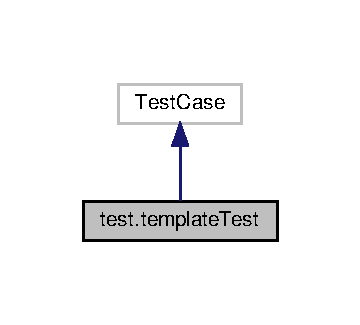
\includegraphics[width=173pt]{classtest_1_1templateTest__inherit__graph}
\end{center}
\end{figure}


Collaboration diagram for test.\+template\+Test\+:\nopagebreak
\begin{figure}[H]
\begin{center}
\leavevmode
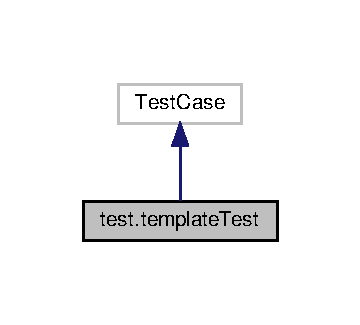
\includegraphics[width=173pt]{classtest_1_1templateTest__coll__graph}
\end{center}
\end{figure}
\subsection*{Public Member Functions}
\begin{DoxyCompactItemize}
\item 
\mbox{\Hypertarget{classtest_1_1templateTest_ad521602ca86084ef419755d76c732dc8}\label{classtest_1_1templateTest_ad521602ca86084ef419755d76c732dc8}} 
def \hyperlink{classtest_1_1templateTest_ad521602ca86084ef419755d76c732dc8}{set\+Up} (self)
\begin{DoxyCompactList}\small\item\em runs before every test \end{DoxyCompactList}\item 
\mbox{\Hypertarget{classtest_1_1templateTest_a85b2889c84ac2b27e4ba38c574d62b9a}\label{classtest_1_1templateTest_a85b2889c84ac2b27e4ba38c574d62b9a}} 
def \hyperlink{classtest_1_1templateTest_a85b2889c84ac2b27e4ba38c574d62b9a}{test\+A\+Equal} (self)
\begin{DoxyCompactList}\small\item\em tests X \end{DoxyCompactList}\item 
def \hyperlink{classtest_1_1templateTest_ae7eca3c8bbe8224c4b8c28bcfeb5d50f}{test\+B\+Exception} (self)
\begin{DoxyCompactList}\small\item\em tests X \end{DoxyCompactList}\end{DoxyCompactItemize}


\subsection{Detailed Description}
Tests. 

\subsection{Member Function Documentation}
\mbox{\Hypertarget{classtest_1_1templateTest_ae7eca3c8bbe8224c4b8c28bcfeb5d50f}\label{classtest_1_1templateTest_ae7eca3c8bbe8224c4b8c28bcfeb5d50f}} 
\index{test\+::template\+Test@{test\+::template\+Test}!test\+B\+Exception@{test\+B\+Exception}}
\index{test\+B\+Exception@{test\+B\+Exception}!test\+::template\+Test@{test\+::template\+Test}}
\subsubsection{\texorpdfstring{test\+B\+Exception()}{testBException()}}
{\footnotesize\ttfamily def test.\+template\+Test.\+test\+B\+Exception (\begin{DoxyParamCaption}\item[{}]{self }\end{DoxyParamCaption})}



tests X 

catches thrown error 

The documentation for this class was generated from the following file\+:\begin{DoxyCompactItemize}
\item 
/home/gab/repos/application\+\_\+3xa3\+\_\+l01\+\_\+grp05/src/\hyperlink{test_8py}{test.\+py}\end{DoxyCompactItemize}

\hypertarget{classuserProfile_1_1userProfile}{}\section{user\+Profile.\+user\+Profile Class Reference}
\label{classuserProfile_1_1userProfile}\index{user\+Profile.\+user\+Profile@{user\+Profile.\+user\+Profile}}


This class represents the preferences of a user for job searching.  


\subsection*{Public Member Functions}
\begin{DoxyCompactItemize}
\item 
def \hyperlink{classuserProfile_1_1userProfile_acc3074e2b18f583f4c29112dc8c7ac10}{\+\_\+\+\_\+init\+\_\+\+\_\+} (self, user\+Prompts=True)
\begin{DoxyCompactList}\small\item\em Constructor for \hyperlink{classuserProfile_1_1userProfile}{user\+Profile}. \end{DoxyCompactList}\item 
def \hyperlink{classuserProfile_1_1userProfile_a7243a67eaec172d035828f95779b9534}{load\+Profile} (self, user\+Prompts=\char`\"{}\char`\"{}, file=\char`\"{}profile.\+yaml\char`\"{})
\begin{DoxyCompactList}\small\item\em Method attempts to load values from the given file to itself. \end{DoxyCompactList}\item 
def \hyperlink{classuserProfile_1_1userProfile_aabe8e582214f44b0315fee65fb97a5a3}{save\+Profile} (self, user\+Prompts=\char`\"{}\char`\"{}, file=\char`\"{}profile.\+yaml\char`\"{})
\begin{DoxyCompactList}\small\item\em Method attempts to save its variable values to the given file. \end{DoxyCompactList}\item 
def \hyperlink{classuserProfile_1_1userProfile_a805c57945934e5b839077ee8d8edfe5d}{is\+Complete} (self, user\+Prompts=\char`\"{}\char`\"{})
\begin{DoxyCompactList}\small\item\em Method verifies that all profile elements were changed that are required for a base job application. \end{DoxyCompactList}\item 
def \hyperlink{classuserProfile_1_1userProfile_a1a61a204207c67cc6bc2c0b2b810ea32}{get\+Keywords} (self)
\begin{DoxyCompactList}\small\item\em Method gets keywords to use in searching. \end{DoxyCompactList}\item 
def \hyperlink{classuserProfile_1_1userProfile_a8cbc67cf93584ff8a9bd0d032c0a1c44}{get\+Job\+Title} (self)
\begin{DoxyCompactList}\small\item\em Method gets job title to use in searching. \end{DoxyCompactList}\item 
def \hyperlink{classuserProfile_1_1userProfile_afa86adbeac8ea685d8c9f1d343f734fd}{get\+Site} (self)
\begin{DoxyCompactList}\small\item\em Method gets site that will be scraped. \end{DoxyCompactList}\item 
def \hyperlink{classuserProfile_1_1userProfile_a3b66b43cf824415acf3c18dfb71ae226}{get\+First\+Name} (self)
\begin{DoxyCompactList}\small\item\em Method gets first name. \end{DoxyCompactList}\item 
def \hyperlink{classuserProfile_1_1userProfile_acb6d2593a392756816a448e09bdc1b24}{get\+Last\+Name} (self)
\begin{DoxyCompactList}\small\item\em Method gets last name. \end{DoxyCompactList}\item 
def \hyperlink{classuserProfile_1_1userProfile_a31aed4505464a0f546e0bb33306a355d}{get\+Email} (self)
\begin{DoxyCompactList}\small\item\em Method gets main contact email. \end{DoxyCompactList}\item 
def \hyperlink{classuserProfile_1_1userProfile_ac6014db8a44e3e1ea44d30a2dbeb2b25}{get\+Phone} (self)
\begin{DoxyCompactList}\small\item\em Method gets phone number. \end{DoxyCompactList}\item 
def \hyperlink{classuserProfile_1_1userProfile_aa146aa6eba2de13cfcff77e14409b891}{get\+Organisation} (self)
\begin{DoxyCompactList}\small\item\em Method gets organisation name. \end{DoxyCompactList}\item 
def \hyperlink{classuserProfile_1_1userProfile_aa89ac2871990f63c02a2bebb3393c979}{get\+Resume\+Path} (self)
\begin{DoxyCompactList}\small\item\em Method gets path to resume file. \end{DoxyCompactList}\item 
def \hyperlink{classuserProfile_1_1userProfile_ab2a8462b4239f832cdc0bc774ca60968}{get\+Socials} (self)
\begin{DoxyCompactList}\small\item\em Method gets social media links. \end{DoxyCompactList}\item 
def \hyperlink{classuserProfile_1_1userProfile_a50577f0100db886c2c5d6cdfc61c73a6}{get\+Location} (self)
\begin{DoxyCompactList}\small\item\em Method gets city, state/province if applicable, and country of residence. \end{DoxyCompactList}\item 
def \hyperlink{classuserProfile_1_1userProfile_acdaf40b01b5086ab70b8802ba944b337}{get\+Grad\+Date} (self)
\begin{DoxyCompactList}\small\item\em Method gets graduation date. \end{DoxyCompactList}\item 
def \hyperlink{classuserProfile_1_1userProfile_a25a425c5045c07739c784f7f8dcff2af}{get\+University} (self)
\begin{DoxyCompactList}\small\item\em Method gets university attended. \end{DoxyCompactList}\item 
def \hyperlink{classuserProfile_1_1userProfile_aa3806d54ee2f967e826537926e5aadf8}{get\+Auto\+Login} (self, convert=True)
\begin{DoxyCompactList}\small\item\em Method gets whether or not website logins should be automated. \end{DoxyCompactList}\item 
def \hyperlink{classuserProfile_1_1userProfile_adb914cd59899ee5fc36c23be7f2219d0}{get\+Profile\+Dict} (self)
\begin{DoxyCompactList}\small\item\em Method gets all values stored in profile. \end{DoxyCompactList}\item 
def \hyperlink{classuserProfile_1_1userProfile_ad1e2dc6aedf50cba360f2bc6669ea3f9}{set\+Keywords} (self, keywords, toggle\+Mode=False)
\begin{DoxyCompactList}\small\item\em Method sets keywords. \end{DoxyCompactList}\item 
def \hyperlink{classuserProfile_1_1userProfile_aa8d7bc0df8fb26fe203b8c6459cd403c}{set\+Job\+Title} (self, title)
\begin{DoxyCompactList}\small\item\em Method sets job title. \end{DoxyCompactList}\item 
def \hyperlink{classuserProfile_1_1userProfile_a67fc7d06910ee0cb4914884dff2ef28e}{set\+Site} (self, site)
\begin{DoxyCompactList}\small\item\em Method tries to set active site for scraping. \end{DoxyCompactList}\item 
def \hyperlink{classuserProfile_1_1userProfile_aafd4f084d296a83fb1ac2ff703aaa251}{set\+First\+Name} (self, name)
\begin{DoxyCompactList}\small\item\em Method sets first name. \end{DoxyCompactList}\item 
def \hyperlink{classuserProfile_1_1userProfile_ab6c77d7b146fbf8d9ffb79ae0d6a2c00}{set\+Last\+Name} (self, name)
\begin{DoxyCompactList}\small\item\em Method sets last name. \end{DoxyCompactList}\item 
def \hyperlink{classuserProfile_1_1userProfile_a6420f8a55919d59d5d357b9ed93cb279}{set\+Email} (self, email)
\begin{DoxyCompactList}\small\item\em Method tries to set email. \end{DoxyCompactList}\item 
def \hyperlink{classuserProfile_1_1userProfile_af57b152c37a8ce53368166751893e0b3}{set\+Phone} (self, phone)
\begin{DoxyCompactList}\small\item\em Method tries to set phone number. \end{DoxyCompactList}\item 
def \hyperlink{classuserProfile_1_1userProfile_a240b062efefc77fb5137306709aef5ed}{set\+Organisation} (self, org)
\begin{DoxyCompactList}\small\item\em Method sets organisation. \end{DoxyCompactList}\item 
def \hyperlink{classuserProfile_1_1userProfile_ae7ad036942595e2ae9c1247d2c49a63b}{set\+Resume\+Path} (self, file, append\+Working=True)
\begin{DoxyCompactList}\small\item\em Method tries to set path to resume file. \end{DoxyCompactList}\item 
def \hyperlink{classuserProfile_1_1userProfile_a2a10347741d3e396e48d6aa1bb49cecb}{set\+Socials} (self, link, toggle\+Mode=False)
\begin{DoxyCompactList}\small\item\em Method sets social links. \end{DoxyCompactList}\item 
def \hyperlink{classuserProfile_1_1userProfile_ad8b26311a1d9adf8b7b29c7d7ab73358}{set\+Location} (self, loc)
\begin{DoxyCompactList}\small\item\em Method sets location. \end{DoxyCompactList}\item 
def \hyperlink{classuserProfile_1_1userProfile_a49e06c1b0a539a79d66108e096fc46d6}{set\+Grad\+Date} (self, grad)
\begin{DoxyCompactList}\small\item\em Method tries to set grad date. \end{DoxyCompactList}\item 
def \hyperlink{classuserProfile_1_1userProfile_a33423b70af186c953dc94e302cc717d3}{set\+University} (self, name)
\begin{DoxyCompactList}\small\item\em Method sets university. \end{DoxyCompactList}\item 
def \hyperlink{classuserProfile_1_1userProfile_a069b4dcc551295eceac4eaef147d59f3}{set\+Auto\+Login} (self, val)
\begin{DoxyCompactList}\small\item\em Method sets auto login setting. \end{DoxyCompactList}\end{DoxyCompactItemize}


\subsection{Detailed Description}
This class represents the preferences of a user for job searching. 

\subsection{Constructor \& Destructor Documentation}
\mbox{\Hypertarget{classuserProfile_1_1userProfile_acc3074e2b18f583f4c29112dc8c7ac10}\label{classuserProfile_1_1userProfile_acc3074e2b18f583f4c29112dc8c7ac10}} 
\index{user\+Profile\+::user\+Profile@{user\+Profile\+::user\+Profile}!\+\_\+\+\_\+init\+\_\+\+\_\+@{\+\_\+\+\_\+init\+\_\+\+\_\+}}
\index{\+\_\+\+\_\+init\+\_\+\+\_\+@{\+\_\+\+\_\+init\+\_\+\+\_\+}!user\+Profile\+::user\+Profile@{user\+Profile\+::user\+Profile}}
\subsubsection{\texorpdfstring{\+\_\+\+\_\+init\+\_\+\+\_\+()}{\_\_init\_\_()}}
{\footnotesize\ttfamily def user\+Profile.\+user\+Profile.\+\_\+\+\_\+init\+\_\+\+\_\+ (\begin{DoxyParamCaption}\item[{}]{self,  }\item[{}]{user\+Prompts = {\ttfamily True} }\end{DoxyParamCaption})}



Constructor for \hyperlink{classuserProfile_1_1userProfile}{user\+Profile}. 

Sets default values for profile 
\begin{DoxyParams}{Parameters}
{\em user\+Prompts} & (optional) Boolean default class value for if user should require confirmations when performing tasks like saving/loading \\
\hline
\end{DoxyParams}


\subsection{Member Function Documentation}
\mbox{\Hypertarget{classuserProfile_1_1userProfile_aa3806d54ee2f967e826537926e5aadf8}\label{classuserProfile_1_1userProfile_aa3806d54ee2f967e826537926e5aadf8}} 
\index{user\+Profile\+::user\+Profile@{user\+Profile\+::user\+Profile}!get\+Auto\+Login@{get\+Auto\+Login}}
\index{get\+Auto\+Login@{get\+Auto\+Login}!user\+Profile\+::user\+Profile@{user\+Profile\+::user\+Profile}}
\subsubsection{\texorpdfstring{get\+Auto\+Login()}{getAutoLogin()}}
{\footnotesize\ttfamily def user\+Profile.\+user\+Profile.\+get\+Auto\+Login (\begin{DoxyParamCaption}\item[{}]{self,  }\item[{}]{convert = {\ttfamily True} }\end{DoxyParamCaption})}



Method gets whether or not website logins should be automated. 


\begin{DoxyParams}{Parameters}
{\em convert} & (optional) Boolean if blank value should be converted to False \\
\hline
\end{DoxyParams}
\begin{DoxyReturn}{Returns}
String indicating name of university 
\end{DoxyReturn}
\mbox{\Hypertarget{classuserProfile_1_1userProfile_a31aed4505464a0f546e0bb33306a355d}\label{classuserProfile_1_1userProfile_a31aed4505464a0f546e0bb33306a355d}} 
\index{user\+Profile\+::user\+Profile@{user\+Profile\+::user\+Profile}!get\+Email@{get\+Email}}
\index{get\+Email@{get\+Email}!user\+Profile\+::user\+Profile@{user\+Profile\+::user\+Profile}}
\subsubsection{\texorpdfstring{get\+Email()}{getEmail()}}
{\footnotesize\ttfamily def user\+Profile.\+user\+Profile.\+get\+Email (\begin{DoxyParamCaption}\item[{}]{self }\end{DoxyParamCaption})}



Method gets main contact email. 

\begin{DoxyReturn}{Returns}
String indicating email address 
\end{DoxyReturn}
\mbox{\Hypertarget{classuserProfile_1_1userProfile_a3b66b43cf824415acf3c18dfb71ae226}\label{classuserProfile_1_1userProfile_a3b66b43cf824415acf3c18dfb71ae226}} 
\index{user\+Profile\+::user\+Profile@{user\+Profile\+::user\+Profile}!get\+First\+Name@{get\+First\+Name}}
\index{get\+First\+Name@{get\+First\+Name}!user\+Profile\+::user\+Profile@{user\+Profile\+::user\+Profile}}
\subsubsection{\texorpdfstring{get\+First\+Name()}{getFirstName()}}
{\footnotesize\ttfamily def user\+Profile.\+user\+Profile.\+get\+First\+Name (\begin{DoxyParamCaption}\item[{}]{self }\end{DoxyParamCaption})}



Method gets first name. 

\begin{DoxyReturn}{Returns}
String indicating first name 
\end{DoxyReturn}
\mbox{\Hypertarget{classuserProfile_1_1userProfile_acdaf40b01b5086ab70b8802ba944b337}\label{classuserProfile_1_1userProfile_acdaf40b01b5086ab70b8802ba944b337}} 
\index{user\+Profile\+::user\+Profile@{user\+Profile\+::user\+Profile}!get\+Grad\+Date@{get\+Grad\+Date}}
\index{get\+Grad\+Date@{get\+Grad\+Date}!user\+Profile\+::user\+Profile@{user\+Profile\+::user\+Profile}}
\subsubsection{\texorpdfstring{get\+Grad\+Date()}{getGradDate()}}
{\footnotesize\ttfamily def user\+Profile.\+user\+Profile.\+get\+Grad\+Date (\begin{DoxyParamCaption}\item[{}]{self }\end{DoxyParamCaption})}



Method gets graduation date. 

\begin{DoxyReturn}{Returns}
Tuple of 2 integers indicating the month and year of graduation 
\end{DoxyReturn}
\mbox{\Hypertarget{classuserProfile_1_1userProfile_a8cbc67cf93584ff8a9bd0d032c0a1c44}\label{classuserProfile_1_1userProfile_a8cbc67cf93584ff8a9bd0d032c0a1c44}} 
\index{user\+Profile\+::user\+Profile@{user\+Profile\+::user\+Profile}!get\+Job\+Title@{get\+Job\+Title}}
\index{get\+Job\+Title@{get\+Job\+Title}!user\+Profile\+::user\+Profile@{user\+Profile\+::user\+Profile}}
\subsubsection{\texorpdfstring{get\+Job\+Title()}{getJobTitle()}}
{\footnotesize\ttfamily def user\+Profile.\+user\+Profile.\+get\+Job\+Title (\begin{DoxyParamCaption}\item[{}]{self }\end{DoxyParamCaption})}



Method gets job title to use in searching. 

\begin{DoxyReturn}{Returns}
String indicating job title 
\end{DoxyReturn}
\mbox{\Hypertarget{classuserProfile_1_1userProfile_a1a61a204207c67cc6bc2c0b2b810ea32}\label{classuserProfile_1_1userProfile_a1a61a204207c67cc6bc2c0b2b810ea32}} 
\index{user\+Profile\+::user\+Profile@{user\+Profile\+::user\+Profile}!get\+Keywords@{get\+Keywords}}
\index{get\+Keywords@{get\+Keywords}!user\+Profile\+::user\+Profile@{user\+Profile\+::user\+Profile}}
\subsubsection{\texorpdfstring{get\+Keywords()}{getKeywords()}}
{\footnotesize\ttfamily def user\+Profile.\+user\+Profile.\+get\+Keywords (\begin{DoxyParamCaption}\item[{}]{self }\end{DoxyParamCaption})}



Method gets keywords to use in searching. 

\begin{DoxyReturn}{Returns}
List of strings indicating keywords 
\end{DoxyReturn}
\mbox{\Hypertarget{classuserProfile_1_1userProfile_acb6d2593a392756816a448e09bdc1b24}\label{classuserProfile_1_1userProfile_acb6d2593a392756816a448e09bdc1b24}} 
\index{user\+Profile\+::user\+Profile@{user\+Profile\+::user\+Profile}!get\+Last\+Name@{get\+Last\+Name}}
\index{get\+Last\+Name@{get\+Last\+Name}!user\+Profile\+::user\+Profile@{user\+Profile\+::user\+Profile}}
\subsubsection{\texorpdfstring{get\+Last\+Name()}{getLastName()}}
{\footnotesize\ttfamily def user\+Profile.\+user\+Profile.\+get\+Last\+Name (\begin{DoxyParamCaption}\item[{}]{self }\end{DoxyParamCaption})}



Method gets last name. 

\begin{DoxyReturn}{Returns}
String indicating last name 
\end{DoxyReturn}
\mbox{\Hypertarget{classuserProfile_1_1userProfile_a50577f0100db886c2c5d6cdfc61c73a6}\label{classuserProfile_1_1userProfile_a50577f0100db886c2c5d6cdfc61c73a6}} 
\index{user\+Profile\+::user\+Profile@{user\+Profile\+::user\+Profile}!get\+Location@{get\+Location}}
\index{get\+Location@{get\+Location}!user\+Profile\+::user\+Profile@{user\+Profile\+::user\+Profile}}
\subsubsection{\texorpdfstring{get\+Location()}{getLocation()}}
{\footnotesize\ttfamily def user\+Profile.\+user\+Profile.\+get\+Location (\begin{DoxyParamCaption}\item[{}]{self }\end{DoxyParamCaption})}



Method gets city, state/province if applicable, and country of residence. 

\begin{DoxyReturn}{Returns}
Tuple of 3 strings indicating city, state/province (empty string if none was provided), and country of residence 
\end{DoxyReturn}
\mbox{\Hypertarget{classuserProfile_1_1userProfile_aa146aa6eba2de13cfcff77e14409b891}\label{classuserProfile_1_1userProfile_aa146aa6eba2de13cfcff77e14409b891}} 
\index{user\+Profile\+::user\+Profile@{user\+Profile\+::user\+Profile}!get\+Organisation@{get\+Organisation}}
\index{get\+Organisation@{get\+Organisation}!user\+Profile\+::user\+Profile@{user\+Profile\+::user\+Profile}}
\subsubsection{\texorpdfstring{get\+Organisation()}{getOrganisation()}}
{\footnotesize\ttfamily def user\+Profile.\+user\+Profile.\+get\+Organisation (\begin{DoxyParamCaption}\item[{}]{self }\end{DoxyParamCaption})}



Method gets organisation name. 

\begin{DoxyReturn}{Returns}
String indicating organisation 
\end{DoxyReturn}
\mbox{\Hypertarget{classuserProfile_1_1userProfile_ac6014db8a44e3e1ea44d30a2dbeb2b25}\label{classuserProfile_1_1userProfile_ac6014db8a44e3e1ea44d30a2dbeb2b25}} 
\index{user\+Profile\+::user\+Profile@{user\+Profile\+::user\+Profile}!get\+Phone@{get\+Phone}}
\index{get\+Phone@{get\+Phone}!user\+Profile\+::user\+Profile@{user\+Profile\+::user\+Profile}}
\subsubsection{\texorpdfstring{get\+Phone()}{getPhone()}}
{\footnotesize\ttfamily def user\+Profile.\+user\+Profile.\+get\+Phone (\begin{DoxyParamCaption}\item[{}]{self }\end{DoxyParamCaption})}



Method gets phone number. 

\begin{DoxyReturn}{Returns}
String of numbers indicating phone number 
\end{DoxyReturn}
\mbox{\Hypertarget{classuserProfile_1_1userProfile_adb914cd59899ee5fc36c23be7f2219d0}\label{classuserProfile_1_1userProfile_adb914cd59899ee5fc36c23be7f2219d0}} 
\index{user\+Profile\+::user\+Profile@{user\+Profile\+::user\+Profile}!get\+Profile\+Dict@{get\+Profile\+Dict}}
\index{get\+Profile\+Dict@{get\+Profile\+Dict}!user\+Profile\+::user\+Profile@{user\+Profile\+::user\+Profile}}
\subsubsection{\texorpdfstring{get\+Profile\+Dict()}{getProfileDict()}}
{\footnotesize\ttfamily def user\+Profile.\+user\+Profile.\+get\+Profile\+Dict (\begin{DoxyParamCaption}\item[{}]{self }\end{DoxyParamCaption})}



Method gets all values stored in profile. 

\begin{DoxyReturn}{Returns}
Dictionary with string keys matching values in profile 
\end{DoxyReturn}
\mbox{\Hypertarget{classuserProfile_1_1userProfile_aa89ac2871990f63c02a2bebb3393c979}\label{classuserProfile_1_1userProfile_aa89ac2871990f63c02a2bebb3393c979}} 
\index{user\+Profile\+::user\+Profile@{user\+Profile\+::user\+Profile}!get\+Resume\+Path@{get\+Resume\+Path}}
\index{get\+Resume\+Path@{get\+Resume\+Path}!user\+Profile\+::user\+Profile@{user\+Profile\+::user\+Profile}}
\subsubsection{\texorpdfstring{get\+Resume\+Path()}{getResumePath()}}
{\footnotesize\ttfamily def user\+Profile.\+user\+Profile.\+get\+Resume\+Path (\begin{DoxyParamCaption}\item[{}]{self }\end{DoxyParamCaption})}



Method gets path to resume file. 

\begin{DoxyReturn}{Returns}
String indicating path to resume file 
\end{DoxyReturn}
\mbox{\Hypertarget{classuserProfile_1_1userProfile_afa86adbeac8ea685d8c9f1d343f734fd}\label{classuserProfile_1_1userProfile_afa86adbeac8ea685d8c9f1d343f734fd}} 
\index{user\+Profile\+::user\+Profile@{user\+Profile\+::user\+Profile}!get\+Site@{get\+Site}}
\index{get\+Site@{get\+Site}!user\+Profile\+::user\+Profile@{user\+Profile\+::user\+Profile}}
\subsubsection{\texorpdfstring{get\+Site()}{getSite()}}
{\footnotesize\ttfamily def user\+Profile.\+user\+Profile.\+get\+Site (\begin{DoxyParamCaption}\item[{}]{self }\end{DoxyParamCaption})}



Method gets site that will be scraped. 

\begin{DoxyReturn}{Returns}
String indicating name of site 
\end{DoxyReturn}
\mbox{\Hypertarget{classuserProfile_1_1userProfile_ab2a8462b4239f832cdc0bc774ca60968}\label{classuserProfile_1_1userProfile_ab2a8462b4239f832cdc0bc774ca60968}} 
\index{user\+Profile\+::user\+Profile@{user\+Profile\+::user\+Profile}!get\+Socials@{get\+Socials}}
\index{get\+Socials@{get\+Socials}!user\+Profile\+::user\+Profile@{user\+Profile\+::user\+Profile}}
\subsubsection{\texorpdfstring{get\+Socials()}{getSocials()}}
{\footnotesize\ttfamily def user\+Profile.\+user\+Profile.\+get\+Socials (\begin{DoxyParamCaption}\item[{}]{self }\end{DoxyParamCaption})}



Method gets social media links. 

\begin{DoxyReturn}{Returns}
List of strings indicating U\+R\+Ls to social media profiles 
\end{DoxyReturn}
\mbox{\Hypertarget{classuserProfile_1_1userProfile_a25a425c5045c07739c784f7f8dcff2af}\label{classuserProfile_1_1userProfile_a25a425c5045c07739c784f7f8dcff2af}} 
\index{user\+Profile\+::user\+Profile@{user\+Profile\+::user\+Profile}!get\+University@{get\+University}}
\index{get\+University@{get\+University}!user\+Profile\+::user\+Profile@{user\+Profile\+::user\+Profile}}
\subsubsection{\texorpdfstring{get\+University()}{getUniversity()}}
{\footnotesize\ttfamily def user\+Profile.\+user\+Profile.\+get\+University (\begin{DoxyParamCaption}\item[{}]{self }\end{DoxyParamCaption})}



Method gets university attended. 

\begin{DoxyReturn}{Returns}
String indicating name of university 
\end{DoxyReturn}
\mbox{\Hypertarget{classuserProfile_1_1userProfile_a805c57945934e5b839077ee8d8edfe5d}\label{classuserProfile_1_1userProfile_a805c57945934e5b839077ee8d8edfe5d}} 
\index{user\+Profile\+::user\+Profile@{user\+Profile\+::user\+Profile}!is\+Complete@{is\+Complete}}
\index{is\+Complete@{is\+Complete}!user\+Profile\+::user\+Profile@{user\+Profile\+::user\+Profile}}
\subsubsection{\texorpdfstring{is\+Complete()}{isComplete()}}
{\footnotesize\ttfamily def user\+Profile.\+user\+Profile.\+is\+Complete (\begin{DoxyParamCaption}\item[{}]{self,  }\item[{}]{user\+Prompts = {\ttfamily \char`\"{}\char`\"{}} }\end{DoxyParamCaption})}



Method verifies that all profile elements were changed that are required for a base job application. 


\begin{DoxyParams}{Parameters}
{\em user\+Prompts} & (optional) Boolean for if user should require confirmations \\
\hline
\end{DoxyParams}
\begin{DoxyReturn}{Returns}
Boolean if required changes have been made 
\end{DoxyReturn}
\mbox{\Hypertarget{classuserProfile_1_1userProfile_a7243a67eaec172d035828f95779b9534}\label{classuserProfile_1_1userProfile_a7243a67eaec172d035828f95779b9534}} 
\index{user\+Profile\+::user\+Profile@{user\+Profile\+::user\+Profile}!load\+Profile@{load\+Profile}}
\index{load\+Profile@{load\+Profile}!user\+Profile\+::user\+Profile@{user\+Profile\+::user\+Profile}}
\subsubsection{\texorpdfstring{load\+Profile()}{loadProfile()}}
{\footnotesize\ttfamily def user\+Profile.\+user\+Profile.\+load\+Profile (\begin{DoxyParamCaption}\item[{}]{self,  }\item[{}]{user\+Prompts = {\ttfamily \char`\"{}\char`\"{}},  }\item[{}]{file = {\ttfamily \char`\"{}profile.yaml\char`\"{}} }\end{DoxyParamCaption})}



Method attempts to load values from the given file to itself. 


\begin{DoxyParams}{Parameters}
{\em user\+Prompts} & (optional) Boolean for if user should require confirmations \\
\hline
{\em file} & (optional) A string of the path to the saved profile \\
\hline
\end{DoxyParams}
\mbox{\Hypertarget{classuserProfile_1_1userProfile_aabe8e582214f44b0315fee65fb97a5a3}\label{classuserProfile_1_1userProfile_aabe8e582214f44b0315fee65fb97a5a3}} 
\index{user\+Profile\+::user\+Profile@{user\+Profile\+::user\+Profile}!save\+Profile@{save\+Profile}}
\index{save\+Profile@{save\+Profile}!user\+Profile\+::user\+Profile@{user\+Profile\+::user\+Profile}}
\subsubsection{\texorpdfstring{save\+Profile()}{saveProfile()}}
{\footnotesize\ttfamily def user\+Profile.\+user\+Profile.\+save\+Profile (\begin{DoxyParamCaption}\item[{}]{self,  }\item[{}]{user\+Prompts = {\ttfamily \char`\"{}\char`\"{}},  }\item[{}]{file = {\ttfamily \char`\"{}profile.yaml\char`\"{}} }\end{DoxyParamCaption})}



Method attempts to save its variable values to the given file. 

Will overwrite the file if it exists already 
\begin{DoxyParams}{Parameters}
{\em user\+Prompts} & (optional) Boolean for if user should require confirmations \\
\hline
{\em file} & (optional) A string indicating a path to the profile to write \\
\hline
\end{DoxyParams}
\mbox{\Hypertarget{classuserProfile_1_1userProfile_a069b4dcc551295eceac4eaef147d59f3}\label{classuserProfile_1_1userProfile_a069b4dcc551295eceac4eaef147d59f3}} 
\index{user\+Profile\+::user\+Profile@{user\+Profile\+::user\+Profile}!set\+Auto\+Login@{set\+Auto\+Login}}
\index{set\+Auto\+Login@{set\+Auto\+Login}!user\+Profile\+::user\+Profile@{user\+Profile\+::user\+Profile}}
\subsubsection{\texorpdfstring{set\+Auto\+Login()}{setAutoLogin()}}
{\footnotesize\ttfamily def user\+Profile.\+user\+Profile.\+set\+Auto\+Login (\begin{DoxyParamCaption}\item[{}]{self,  }\item[{}]{val }\end{DoxyParamCaption})}



Method sets auto login setting. 


\begin{DoxyParams}{Parameters}
{\em val} & Boolean indicating if auto login should be done \\
\hline
\end{DoxyParams}
\mbox{\Hypertarget{classuserProfile_1_1userProfile_a6420f8a55919d59d5d357b9ed93cb279}\label{classuserProfile_1_1userProfile_a6420f8a55919d59d5d357b9ed93cb279}} 
\index{user\+Profile\+::user\+Profile@{user\+Profile\+::user\+Profile}!set\+Email@{set\+Email}}
\index{set\+Email@{set\+Email}!user\+Profile\+::user\+Profile@{user\+Profile\+::user\+Profile}}
\subsubsection{\texorpdfstring{set\+Email()}{setEmail()}}
{\footnotesize\ttfamily def user\+Profile.\+user\+Profile.\+set\+Email (\begin{DoxyParamCaption}\item[{}]{self,  }\item[{}]{email }\end{DoxyParamCaption})}



Method tries to set email. 

Method will not change the value if the new input is invalid 
\begin{DoxyParams}{Parameters}
{\em email} & String indicating email \\
\hline
\end{DoxyParams}
\begin{DoxyReturn}{Returns}
Boolean True if email was updated, False if not 
\end{DoxyReturn}
\mbox{\Hypertarget{classuserProfile_1_1userProfile_aafd4f084d296a83fb1ac2ff703aaa251}\label{classuserProfile_1_1userProfile_aafd4f084d296a83fb1ac2ff703aaa251}} 
\index{user\+Profile\+::user\+Profile@{user\+Profile\+::user\+Profile}!set\+First\+Name@{set\+First\+Name}}
\index{set\+First\+Name@{set\+First\+Name}!user\+Profile\+::user\+Profile@{user\+Profile\+::user\+Profile}}
\subsubsection{\texorpdfstring{set\+First\+Name()}{setFirstName()}}
{\footnotesize\ttfamily def user\+Profile.\+user\+Profile.\+set\+First\+Name (\begin{DoxyParamCaption}\item[{}]{self,  }\item[{}]{name }\end{DoxyParamCaption})}



Method sets first name. 


\begin{DoxyParams}{Parameters}
{\em name} & String indicating name \\
\hline
\end{DoxyParams}
\mbox{\Hypertarget{classuserProfile_1_1userProfile_a49e06c1b0a539a79d66108e096fc46d6}\label{classuserProfile_1_1userProfile_a49e06c1b0a539a79d66108e096fc46d6}} 
\index{user\+Profile\+::user\+Profile@{user\+Profile\+::user\+Profile}!set\+Grad\+Date@{set\+Grad\+Date}}
\index{set\+Grad\+Date@{set\+Grad\+Date}!user\+Profile\+::user\+Profile@{user\+Profile\+::user\+Profile}}
\subsubsection{\texorpdfstring{set\+Grad\+Date()}{setGradDate()}}
{\footnotesize\ttfamily def user\+Profile.\+user\+Profile.\+set\+Grad\+Date (\begin{DoxyParamCaption}\item[{}]{self,  }\item[{}]{grad }\end{DoxyParamCaption})}



Method tries to set grad date. 


\begin{DoxyParams}{Parameters}
{\em grad} & A length 2 list of strings indicating a month (as name or int) and year \\
\hline
\end{DoxyParams}
\begin{DoxyReturn}{Returns}
Boolean True if date was updated, False if not 
\end{DoxyReturn}
\mbox{\Hypertarget{classuserProfile_1_1userProfile_aa8d7bc0df8fb26fe203b8c6459cd403c}\label{classuserProfile_1_1userProfile_aa8d7bc0df8fb26fe203b8c6459cd403c}} 
\index{user\+Profile\+::user\+Profile@{user\+Profile\+::user\+Profile}!set\+Job\+Title@{set\+Job\+Title}}
\index{set\+Job\+Title@{set\+Job\+Title}!user\+Profile\+::user\+Profile@{user\+Profile\+::user\+Profile}}
\subsubsection{\texorpdfstring{set\+Job\+Title()}{setJobTitle()}}
{\footnotesize\ttfamily def user\+Profile.\+user\+Profile.\+set\+Job\+Title (\begin{DoxyParamCaption}\item[{}]{self,  }\item[{}]{title }\end{DoxyParamCaption})}



Method sets job title. 


\begin{DoxyParams}{Parameters}
{\em name} & String indicating job title \\
\hline
\end{DoxyParams}
\mbox{\Hypertarget{classuserProfile_1_1userProfile_ad1e2dc6aedf50cba360f2bc6669ea3f9}\label{classuserProfile_1_1userProfile_ad1e2dc6aedf50cba360f2bc6669ea3f9}} 
\index{user\+Profile\+::user\+Profile@{user\+Profile\+::user\+Profile}!set\+Keywords@{set\+Keywords}}
\index{set\+Keywords@{set\+Keywords}!user\+Profile\+::user\+Profile@{user\+Profile\+::user\+Profile}}
\subsubsection{\texorpdfstring{set\+Keywords()}{setKeywords()}}
{\footnotesize\ttfamily def user\+Profile.\+user\+Profile.\+set\+Keywords (\begin{DoxyParamCaption}\item[{}]{self,  }\item[{}]{keywords,  }\item[{}]{toggle\+Mode = {\ttfamily False} }\end{DoxyParamCaption})}



Method sets keywords. 


\begin{DoxyParams}{Parameters}
{\em keywords} & A list of strings used as keywords \\
\hline
{\em toggle\+Mode} & (optional) If true, instead of overwriting the class varible with the parameter, it will add words to the class varable from the parameter that are not there and remove ones that are \\
\hline
\end{DoxyParams}
\mbox{\Hypertarget{classuserProfile_1_1userProfile_ab6c77d7b146fbf8d9ffb79ae0d6a2c00}\label{classuserProfile_1_1userProfile_ab6c77d7b146fbf8d9ffb79ae0d6a2c00}} 
\index{user\+Profile\+::user\+Profile@{user\+Profile\+::user\+Profile}!set\+Last\+Name@{set\+Last\+Name}}
\index{set\+Last\+Name@{set\+Last\+Name}!user\+Profile\+::user\+Profile@{user\+Profile\+::user\+Profile}}
\subsubsection{\texorpdfstring{set\+Last\+Name()}{setLastName()}}
{\footnotesize\ttfamily def user\+Profile.\+user\+Profile.\+set\+Last\+Name (\begin{DoxyParamCaption}\item[{}]{self,  }\item[{}]{name }\end{DoxyParamCaption})}



Method sets last name. 


\begin{DoxyParams}{Parameters}
{\em name} & String indicating name \\
\hline
\end{DoxyParams}
\mbox{\Hypertarget{classuserProfile_1_1userProfile_ad8b26311a1d9adf8b7b29c7d7ab73358}\label{classuserProfile_1_1userProfile_ad8b26311a1d9adf8b7b29c7d7ab73358}} 
\index{user\+Profile\+::user\+Profile@{user\+Profile\+::user\+Profile}!set\+Location@{set\+Location}}
\index{set\+Location@{set\+Location}!user\+Profile\+::user\+Profile@{user\+Profile\+::user\+Profile}}
\subsubsection{\texorpdfstring{set\+Location()}{setLocation()}}
{\footnotesize\ttfamily def user\+Profile.\+user\+Profile.\+set\+Location (\begin{DoxyParamCaption}\item[{}]{self,  }\item[{}]{loc }\end{DoxyParamCaption})}



Method sets location. 

If 2 inputs received, it will be stored as a length 3 with a blank value between the two inputted values so indexing always access the same kind of location (i.\+e. country at 2) 
\begin{DoxyParams}{Parameters}
{\em loc} & A length 2 or 3 list of strings indicating locations in the form \mbox{[}city, state/province, country\mbox{]} or \mbox{[}city, country\mbox{]} \\
\hline
\end{DoxyParams}
\begin{DoxyReturn}{Returns}
Boolean True if location was updated, False if not 
\end{DoxyReturn}
\mbox{\Hypertarget{classuserProfile_1_1userProfile_a240b062efefc77fb5137306709aef5ed}\label{classuserProfile_1_1userProfile_a240b062efefc77fb5137306709aef5ed}} 
\index{user\+Profile\+::user\+Profile@{user\+Profile\+::user\+Profile}!set\+Organisation@{set\+Organisation}}
\index{set\+Organisation@{set\+Organisation}!user\+Profile\+::user\+Profile@{user\+Profile\+::user\+Profile}}
\subsubsection{\texorpdfstring{set\+Organisation()}{setOrganisation()}}
{\footnotesize\ttfamily def user\+Profile.\+user\+Profile.\+set\+Organisation (\begin{DoxyParamCaption}\item[{}]{self,  }\item[{}]{org }\end{DoxyParamCaption})}



Method sets organisation. 


\begin{DoxyParams}{Parameters}
{\em org} & String indicating organisation name \\
\hline
\end{DoxyParams}
\mbox{\Hypertarget{classuserProfile_1_1userProfile_af57b152c37a8ce53368166751893e0b3}\label{classuserProfile_1_1userProfile_af57b152c37a8ce53368166751893e0b3}} 
\index{user\+Profile\+::user\+Profile@{user\+Profile\+::user\+Profile}!set\+Phone@{set\+Phone}}
\index{set\+Phone@{set\+Phone}!user\+Profile\+::user\+Profile@{user\+Profile\+::user\+Profile}}
\subsubsection{\texorpdfstring{set\+Phone()}{setPhone()}}
{\footnotesize\ttfamily def user\+Profile.\+user\+Profile.\+set\+Phone (\begin{DoxyParamCaption}\item[{}]{self,  }\item[{}]{phone }\end{DoxyParamCaption})}



Method tries to set phone number. 

Method will not change the value if the new input is invalid; accepts different formats including those with brackets or dashes; do not include country codes 
\begin{DoxyParams}{Parameters}
{\em phone} & String of numbers indicating email \\
\hline
\end{DoxyParams}
\begin{DoxyReturn}{Returns}
Boolean True if email was updated, False if not 
\end{DoxyReturn}
\mbox{\Hypertarget{classuserProfile_1_1userProfile_ae7ad036942595e2ae9c1247d2c49a63b}\label{classuserProfile_1_1userProfile_ae7ad036942595e2ae9c1247d2c49a63b}} 
\index{user\+Profile\+::user\+Profile@{user\+Profile\+::user\+Profile}!set\+Resume\+Path@{set\+Resume\+Path}}
\index{set\+Resume\+Path@{set\+Resume\+Path}!user\+Profile\+::user\+Profile@{user\+Profile\+::user\+Profile}}
\subsubsection{\texorpdfstring{set\+Resume\+Path()}{setResumePath()}}
{\footnotesize\ttfamily def user\+Profile.\+user\+Profile.\+set\+Resume\+Path (\begin{DoxyParamCaption}\item[{}]{self,  }\item[{}]{file,  }\item[{}]{append\+Working = {\ttfamily True} }\end{DoxyParamCaption})}



Method tries to set path to resume file. 

Method also checks if file exists, and if it does not it will not change it 
\begin{DoxyParams}{Parameters}
{\em file} & A string indicating a path to a resume file \\
\hline
{\em append\+Working} & (optional) Append the working directory to the file if applicable \\
\hline
\end{DoxyParams}
\begin{DoxyReturn}{Returns}
Boolean True if file exists and updates, False if not 
\end{DoxyReturn}
\mbox{\Hypertarget{classuserProfile_1_1userProfile_a67fc7d06910ee0cb4914884dff2ef28e}\label{classuserProfile_1_1userProfile_a67fc7d06910ee0cb4914884dff2ef28e}} 
\index{user\+Profile\+::user\+Profile@{user\+Profile\+::user\+Profile}!set\+Site@{set\+Site}}
\index{set\+Site@{set\+Site}!user\+Profile\+::user\+Profile@{user\+Profile\+::user\+Profile}}
\subsubsection{\texorpdfstring{set\+Site()}{setSite()}}
{\footnotesize\ttfamily def user\+Profile.\+user\+Profile.\+set\+Site (\begin{DoxyParamCaption}\item[{}]{self,  }\item[{}]{site }\end{DoxyParamCaption})}



Method tries to set active site for scraping. 

Method will not change the active site if it does not map to one in the list 
\begin{DoxyParams}{Parameters}
{\em site} & Integer inicating index of site to swap to \\
\hline
\end{DoxyParams}
\begin{DoxyReturn}{Returns}
Boolean True if the site was updated, False if not 
\end{DoxyReturn}
\mbox{\Hypertarget{classuserProfile_1_1userProfile_a2a10347741d3e396e48d6aa1bb49cecb}\label{classuserProfile_1_1userProfile_a2a10347741d3e396e48d6aa1bb49cecb}} 
\index{user\+Profile\+::user\+Profile@{user\+Profile\+::user\+Profile}!set\+Socials@{set\+Socials}}
\index{set\+Socials@{set\+Socials}!user\+Profile\+::user\+Profile@{user\+Profile\+::user\+Profile}}
\subsubsection{\texorpdfstring{set\+Socials()}{setSocials()}}
{\footnotesize\ttfamily def user\+Profile.\+user\+Profile.\+set\+Socials (\begin{DoxyParamCaption}\item[{}]{self,  }\item[{}]{link,  }\item[{}]{toggle\+Mode = {\ttfamily False} }\end{DoxyParamCaption})}



Method sets social links. 

When toggle\+Mode = True, only the site name is required to remove an element 
\begin{DoxyParams}{Parameters}
{\em link} & A string representing a link \\
\hline
{\em toggle\+Mode} & (optional) If true, instead of overwriting the class varible with the parameter, it will add words to the class varable from the parameter that are not there and remove ones that are \\
\hline
\end{DoxyParams}
\mbox{\Hypertarget{classuserProfile_1_1userProfile_a33423b70af186c953dc94e302cc717d3}\label{classuserProfile_1_1userProfile_a33423b70af186c953dc94e302cc717d3}} 
\index{user\+Profile\+::user\+Profile@{user\+Profile\+::user\+Profile}!set\+University@{set\+University}}
\index{set\+University@{set\+University}!user\+Profile\+::user\+Profile@{user\+Profile\+::user\+Profile}}
\subsubsection{\texorpdfstring{set\+University()}{setUniversity()}}
{\footnotesize\ttfamily def user\+Profile.\+user\+Profile.\+set\+University (\begin{DoxyParamCaption}\item[{}]{self,  }\item[{}]{name }\end{DoxyParamCaption})}



Method sets university. 


\begin{DoxyParams}{Parameters}
{\em name} & String indicating university name \\
\hline
\end{DoxyParams}


The documentation for this class was generated from the following file\+:\begin{DoxyCompactItemize}
\item 
/home/gab/repos/application\+\_\+3xa3\+\_\+l01\+\_\+grp05/src/\hyperlink{userProfile_8py}{user\+Profile.\+py}\end{DoxyCompactItemize}

\hypertarget{classtest_1_1userProfileBase}{}\section{test.\+user\+Profile\+Base Class Reference}
\label{classtest_1_1userProfileBase}\index{test.\+user\+Profile\+Base@{test.\+user\+Profile\+Base}}


Setup for user\+Profile module.  




Inheritance diagram for test.\+user\+Profile\+Base\+:\nopagebreak
\begin{figure}[H]
\begin{center}
\leavevmode
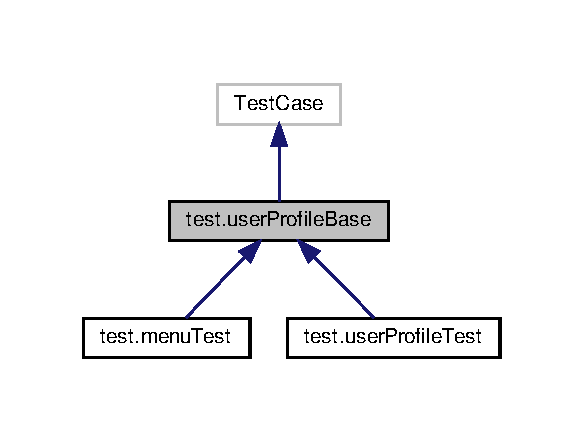
\includegraphics[width=185pt]{classtest_1_1userProfileBase__inherit__graph}
\end{center}
\end{figure}


Collaboration diagram for test.\+user\+Profile\+Base\+:\nopagebreak
\begin{figure}[H]
\begin{center}
\leavevmode
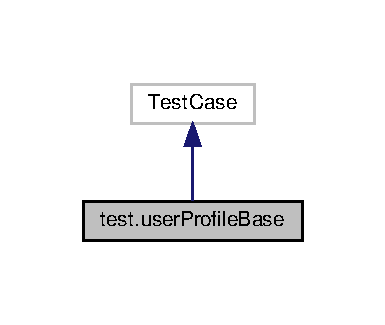
\includegraphics[width=185pt]{classtest_1_1userProfileBase__coll__graph}
\end{center}
\end{figure}
\subsection*{Public Member Functions}
\begin{DoxyCompactItemize}
\item 
\mbox{\Hypertarget{classtest_1_1userProfileBase_ab1675872398acef5e0fede36dd3db672}\label{classtest_1_1userProfileBase_ab1675872398acef5e0fede36dd3db672}} 
def \hyperlink{classtest_1_1userProfileBase_ab1675872398acef5e0fede36dd3db672}{set\+Up} (self)
\begin{DoxyCompactList}\small\item\em Runs before every test. \end{DoxyCompactList}\item 
\mbox{\Hypertarget{classtest_1_1userProfileBase_af6036c1beb54b38dd9d9fb1293aeb3b3}\label{classtest_1_1userProfileBase_af6036c1beb54b38dd9d9fb1293aeb3b3}} 
def \hyperlink{classtest_1_1userProfileBase_af6036c1beb54b38dd9d9fb1293aeb3b3}{load\+Full} (self)
\begin{DoxyCompactList}\small\item\em Fills in profile with non-\/default values. \end{DoxyCompactList}\item 
\mbox{\Hypertarget{classtest_1_1userProfileBase_ac395fc9b444a49856d520874a3b4e90b}\label{classtest_1_1userProfileBase_ac395fc9b444a49856d520874a3b4e90b}} 
def \hyperlink{classtest_1_1userProfileBase_ac395fc9b444a49856d520874a3b4e90b}{make\+Full\+Profile} (self)
\begin{DoxyCompactList}\small\item\em Creates saved profile file for test purposes. \end{DoxyCompactList}\end{DoxyCompactItemize}
\subsection*{Public Attributes}
\begin{DoxyCompactItemize}
\item 
\mbox{\Hypertarget{classtest_1_1userProfileBase_aa2e266103d1680856e874535c72c5988}\label{classtest_1_1userProfileBase_aa2e266103d1680856e874535c72c5988}} 
{\bfseries profile}
\end{DoxyCompactItemize}


\subsection{Detailed Description}
Setup for user\+Profile module. 

The documentation for this class was generated from the following file\+:\begin{DoxyCompactItemize}
\item 
/home/gab/repos/application\+\_\+3xa3\+\_\+l01\+\_\+grp05/src/\hyperlink{test_8py}{test.\+py}\end{DoxyCompactItemize}

\hypertarget{classtest_1_1userProfileTest}{}\section{test.\+user\+Profile\+Test Class Reference}
\label{classtest_1_1userProfileTest}\index{test.\+user\+Profile\+Test@{test.\+user\+Profile\+Test}}


Tests for user\+Profile module.  




Inheritance diagram for test.\+user\+Profile\+Test\+:
\nopagebreak
\begin{figure}[H]
\begin{center}
\leavevmode
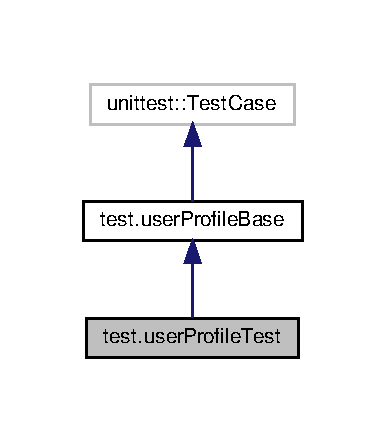
\includegraphics[width=185pt]{classtest_1_1userProfileTest__inherit__graph}
\end{center}
\end{figure}


Collaboration diagram for test.\+user\+Profile\+Test\+:
\nopagebreak
\begin{figure}[H]
\begin{center}
\leavevmode
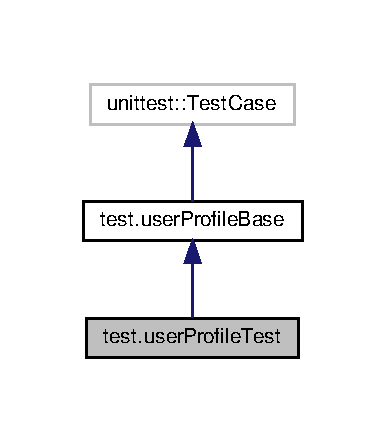
\includegraphics[width=185pt]{classtest_1_1userProfileTest__coll__graph}
\end{center}
\end{figure}
\subsection*{Public Member Functions}
\begin{DoxyCompactItemize}
\item 
\mbox{\Hypertarget{classtest_1_1userProfileTest_a7c8e7b76a66aa454e25ac013af9d2197}\label{classtest_1_1userProfileTest_a7c8e7b76a66aa454e25ac013af9d2197}} 
def \hyperlink{classtest_1_1userProfileTest_a7c8e7b76a66aa454e25ac013af9d2197}{test\+A\+Equal} (self)
\begin{DoxyCompactList}\small\item\em tests X \end{DoxyCompactList}\item 
def \hyperlink{classtest_1_1userProfileTest_a0c63611780a9c06e519e95e82d4794ce}{test\+B\+Exception} (self)
\begin{DoxyCompactList}\small\item\em tests X \end{DoxyCompactList}\end{DoxyCompactItemize}
\subsection*{Additional Inherited Members}


\subsection{Detailed Description}
Tests for user\+Profile module. 

\subsection{Member Function Documentation}
\mbox{\Hypertarget{classtest_1_1userProfileTest_a0c63611780a9c06e519e95e82d4794ce}\label{classtest_1_1userProfileTest_a0c63611780a9c06e519e95e82d4794ce}} 
\index{test\+::user\+Profile\+Test@{test\+::user\+Profile\+Test}!test\+B\+Exception@{test\+B\+Exception}}
\index{test\+B\+Exception@{test\+B\+Exception}!test\+::user\+Profile\+Test@{test\+::user\+Profile\+Test}}
\subsubsection{\texorpdfstring{test\+B\+Exception()}{testBException()}}
{\footnotesize\ttfamily def test.\+user\+Profile\+Test.\+test\+B\+Exception (\begin{DoxyParamCaption}\item[{}]{self }\end{DoxyParamCaption})}



tests X 

catches thrown error 

The documentation for this class was generated from the following file\+:\begin{DoxyCompactItemize}
\item 
/home/gab/repos/application\+\_\+3xa3\+\_\+l01\+\_\+grp05/src/\hyperlink{test_8py}{test.\+py}\end{DoxyCompactItemize}

\chapter{File Documentation}
\hypertarget{apply_8py}{}\section{/home/gab/repos/application\+\_\+3xa3\+\_\+l01\+\_\+grp05/src/apply.py File Reference}
\label{apply_8py}\index{/home/gab/repos/application\+\_\+3xa3\+\_\+l01\+\_\+grp05/src/apply.\+py@{/home/gab/repos/application\+\_\+3xa3\+\_\+l01\+\_\+grp05/src/apply.\+py}}


Main module used for the application proccess.  


\subsection*{Functions}
\begin{DoxyCompactItemize}
\item 
def \hyperlink{apply_8py_ad12e4221cac8a18b0fdd5df5da7f038a}{apply.\+greenhouse} (driver)
\begin{DoxyCompactList}\small\item\em Fills in website text boxes with user information and submits resume. \end{DoxyCompactList}\item 
def \hyperlink{apply_8py_a00006462ba314126513d925b52b7e9e5}{apply.\+lever} (driver)
\begin{DoxyCompactList}\small\item\em Fills in website text boxes with user information and submits resume. \end{DoxyCompactList}\end{DoxyCompactItemize}
\subsection*{Variables}
\begin{DoxyCompactItemize}
\item 
\mbox{\Hypertarget{apply_8py_aaa4d4bf0c2f7b56f3fd71111b98cb75b}\label{apply_8py_aaa4d4bf0c2f7b56f3fd71111b98cb75b}} 
string \hyperlink{apply_8py_aaa4d4bf0c2f7b56f3fd71111b98cb75b}{apply.\+U\+R\+L\+\_\+l2} = \textquotesingle{}https\+://jobs.\+lever.\+co/scratch/2f09a461-\/f01d-\/4041-\/a369-\/c64c1887ed97/apply?lever-\/source=\+Glassdoor\textquotesingle{}
\begin{DoxyCompactList}\small\item\em Global Variables. \end{DoxyCompactList}\item 
\mbox{\Hypertarget{apply_8py_aa3eb038bb4ca5cccf6b295f6a6a7ca37}\label{apply_8py_aa3eb038bb4ca5cccf6b295f6a6a7ca37}} 
string {\bfseries apply.\+U\+R\+L\+\_\+l3} = \textquotesingle{}https\+://jobs.\+lever.\+co/fleetsmith/eb6648a6-\/7ad9-\/4f4a-\/9918-\/8b124e10c525/apply?lever-\/source=\+Glassdoor\textquotesingle{}
\item 
\mbox{\Hypertarget{apply_8py_a365c79d1111144be4705686e25b80463}\label{apply_8py_a365c79d1111144be4705686e25b80463}} 
string {\bfseries apply.\+U\+R\+L\+\_\+l4} = \textquotesingle{}https\+://jobs.\+lever.\+co/stellar/0e5a506b-\/1964-\/40b4-\/93ab-\/31a1ee4e4f90/apply?lever-\/source=\+Glassdoor\textquotesingle{}
\item 
\mbox{\Hypertarget{apply_8py_a46aa7945459d072280a090b0e6d925b6}\label{apply_8py_a46aa7945459d072280a090b0e6d925b6}} 
string {\bfseries apply.\+U\+R\+L\+\_\+l6} = \textquotesingle{}https\+://jobs.\+lever.\+co/verkada/29c66147-\/82ef-\/4293-\/9a6a-\/aeed7e6d619e/apply?lever-\/source=\+Glassdoor\textquotesingle{}
\item 
\mbox{\Hypertarget{apply_8py_afcf31f4e1555dd7666296259fa964eee}\label{apply_8py_afcf31f4e1555dd7666296259fa964eee}} 
string {\bfseries apply.\+U\+R\+L\+\_\+l8} = \textquotesingle{}https\+://jobs.\+lever.\+co/rimeto/bdca896f-\/e7e7-\/4f27-\/a894-\/41b47c729c63/apply?lever-\/source=\+Glassdoor\textquotesingle{}
\item 
\mbox{\Hypertarget{apply_8py_ac5d851198fe2d0f0e783d8959f473366}\label{apply_8py_ac5d851198fe2d0f0e783d8959f473366}} 
string {\bfseries apply.\+U\+R\+L\+\_\+l9} = \textquotesingle{}https\+://jobs.\+lever.\+co/color/20ea56b8-\/fed2-\/413c-\/982d-\/6173e336d51c/apply?lever-\/source=\+Glassdoor\textquotesingle{}
\item 
\mbox{\Hypertarget{apply_8py_a55b98013bfe9662c407216c74afcd4c7}\label{apply_8py_a55b98013bfe9662c407216c74afcd4c7}} 
string {\bfseries apply.\+U\+R\+L\+\_\+g1} = \textquotesingle{}https\+://boards.\+greenhouse.\+io/instabase/jobs/4729606002?utm\+\_\+campaign=google\+\_\+jobs\+\_\+apply\&utm\+\_\+source=google\+\_\+jobs\+\_\+apply\&utm\+\_\+medium=organic\textquotesingle{}
\item 
\mbox{\Hypertarget{apply_8py_ab2cfad3f637ee48a83dc34c1a48504df}\label{apply_8py_ab2cfad3f637ee48a83dc34c1a48504df}} 
list {\bfseries apply.\+U\+R\+LS} = \mbox{[}U\+R\+L\+\_\+g1, U\+R\+L\+\_\+l4, U\+R\+L\+\_\+l3, U\+R\+L\+\_\+l6, U\+R\+L\+\_\+l8, U\+R\+L\+\_\+l9\mbox{]}
\item 
dictionary {\bfseries apply.\+J\+O\+B\+\_\+\+A\+PP}
\item 
\hyperlink{apply_8py_a28be50c998760a690057e2998d1f2a6f}{apply.\+profile} = user\+Profile()
\begin{DoxyCompactList}\small\item\em Initial function run upon execution of program. \end{DoxyCompactList}\item 
\mbox{\Hypertarget{apply_8py_a01d2ff9cd06b1727e62b986ca2d1e0bf}\label{apply_8py_a01d2ff9cd06b1727e62b986ca2d1e0bf}} 
{\bfseries apply.\+site} = profile.\+get\+Site()
\item 
\mbox{\Hypertarget{apply_8py_a994f267a59bfa1915cd92c54bf9ccc66}\label{apply_8py_a994f267a59bfa1915cd92c54bf9ccc66}} 
\hyperlink{apply_8py_a994f267a59bfa1915cd92c54bf9ccc66}{apply.\+aggregated\+U\+R\+Ls} = get\+\_\+links\+\_\+glassdoor.\+get\+U\+R\+Ls()
\begin{DoxyCompactList}\small\item\em Get Links From User Specified Website. \end{DoxyCompactList}\item 
\mbox{\Hypertarget{apply_8py_a934eb0a16e16d7bd0dcbb968fab260a4}\label{apply_8py_a934eb0a16e16d7bd0dcbb968fab260a4}} 
{\bfseries apply.\+driver} = webdriver.\+Chrome(executable\+\_\+path=\textquotesingle{}./chromedriver\textquotesingle{})
\end{DoxyCompactItemize}


\subsection{Detailed Description}
Main module used for the application proccess. 

\begin{DoxyAuthor}{Author}
Gavin Jameson 

Jeremy Langner 

Sam Gorman 
\end{DoxyAuthor}
\begin{DoxyDate}{Date}
Mar 17, 2022 
\end{DoxyDate}


\subsection{Function Documentation}
\mbox{\Hypertarget{apply_8py_file_ad12e4221cac8a18b0fdd5df5da7f038a}\label{apply_8py_file_ad12e4221cac8a18b0fdd5df5da7f038a}} 
\index{apply.\+py@{apply.\+py}!greenhouse@{greenhouse}}
\index{greenhouse@{greenhouse}!apply.\+py@{apply.\+py}}
\subsubsection{\texorpdfstring{greenhouse()}{greenhouse()}}
{\footnotesize\ttfamily def apply.\+greenhouse (\begin{DoxyParamCaption}\item[{}]{driver }\end{DoxyParamCaption})}



Fills in website text boxes with user information and submits resume. 


\begin{DoxyParams}{Parameters}
{\em driver} & Webdriver for chrome which parses and interacts with the H\+T\+ML from a given website \\
\hline
\end{DoxyParams}
\mbox{\Hypertarget{apply_8py_file_a00006462ba314126513d925b52b7e9e5}\label{apply_8py_file_a00006462ba314126513d925b52b7e9e5}} 
\index{apply.\+py@{apply.\+py}!lever@{lever}}
\index{lever@{lever}!apply.\+py@{apply.\+py}}
\subsubsection{\texorpdfstring{lever()}{lever()}}
{\footnotesize\ttfamily def apply.\+lever (\begin{DoxyParamCaption}\item[{}]{driver }\end{DoxyParamCaption})}



Fills in website text boxes with user information and submits resume. 


\begin{DoxyParams}{Parameters}
{\em driver} & Webdriver for chrome which parses and interacts with the H\+T\+ML from a given website \\
\hline
\end{DoxyParams}


\subsection{Variable Documentation}
\mbox{\Hypertarget{apply_8py_file_ae9bedeb7feb9f729a8bdc73dd3555892}\label{apply_8py_file_ae9bedeb7feb9f729a8bdc73dd3555892}} 
\index{apply.\+py@{apply.\+py}!J\+O\+B\+\_\+\+A\+PP@{J\+O\+B\+\_\+\+A\+PP}}
\index{J\+O\+B\+\_\+\+A\+PP@{J\+O\+B\+\_\+\+A\+PP}!apply.\+py@{apply.\+py}}
\subsubsection{\texorpdfstring{J\+O\+B\+\_\+\+A\+PP}{JOB\_APP}}
{\footnotesize\ttfamily dictionary apply.\+J\+O\+B\+\_\+\+A\+PP}

{\bfseries Initial value\+:}
\begin{DoxyCode}
1 =  \{
2     \textcolor{stringliteral}{"first\_name"}: \textcolor{stringliteral}{"Foo"},
3     \textcolor{stringliteral}{"last\_name"}: \textcolor{stringliteral}{"Bar"},
4     \textcolor{stringliteral}{"email"}: \textcolor{stringliteral}{"test@test.com"},
5     \textcolor{stringliteral}{"phone"}: \textcolor{stringliteral}{"123-456-7890"},
6     \textcolor{stringliteral}{"org"}: \textcolor{stringliteral}{"Self-Employed"},
7     \textcolor{stringliteral}{"resume"}: \textcolor{stringliteral}{"resume.pdf"},
8     \textcolor{stringliteral}{"resume\_textfile"}: \textcolor{stringliteral}{"resume\_short.txt"},
9     \textcolor{stringliteral}{"linkedin"}: \textcolor{stringliteral}{"https://www.linkedin.com/"},
10     \textcolor{stringliteral}{"website"}: \textcolor{stringliteral}{"www.youtube.com"},
11     \textcolor{stringliteral}{"github"}: \textcolor{stringliteral}{"https://github.com"},
12     \textcolor{stringliteral}{"twitter"}: \textcolor{stringliteral}{"www.twitter.com"},
13     \textcolor{stringliteral}{"location"}: \textcolor{stringliteral}{"San Francisco, California, United States"},
14     \textcolor{stringliteral}{"grad\_month"}: \textcolor{stringliteral}{'06'},
15     \textcolor{stringliteral}{"grad\_year"}: \textcolor{stringliteral}{'2021'},
16     \textcolor{stringliteral}{"university"}: \textcolor{stringliteral}{"MIT"}
17 \}
\end{DoxyCode}
\mbox{\Hypertarget{apply_8py_file_a28be50c998760a690057e2998d1f2a6f}\label{apply_8py_file_a28be50c998760a690057e2998d1f2a6f}} 
\index{apply.\+py@{apply.\+py}!profile@{profile}}
\index{profile@{profile}!apply.\+py@{apply.\+py}}
\subsubsection{\texorpdfstring{profile}{profile}}
{\footnotesize\ttfamily apply.\+profile = user\+Profile()}



Initial function run upon execution of program. 

Gathers links through secondary modules then coordinates the apllication process 
\hypertarget{get__links__glassdoor_8py}{}\section{/home/gab/repos/application\+\_\+3xa3\+\_\+l01\+\_\+grp05/src/get\+\_\+links\+\_\+glassdoor.py File Reference}
\label{get__links__glassdoor_8py}\index{/home/gab/repos/application\+\_\+3xa3\+\_\+l01\+\_\+grp05/src/get\+\_\+links\+\_\+glassdoor.\+py@{/home/gab/repos/application\+\_\+3xa3\+\_\+l01\+\_\+grp05/src/get\+\_\+links\+\_\+glassdoor.\+py}}


Module used for collecting links from the Glassdoor site.  


\subsection*{Functions}
\begin{DoxyCompactItemize}
\item 
def \hyperlink{get__links__glassdoor_8py_aee0bfbbdba3064819c86ac09d649bb18}{get\+\_\+links\+\_\+glassdoor.\+login} (driver)
\begin{DoxyCompactList}\small\item\em Helper method which gives the user time to log into Glassdoor. \end{DoxyCompactList}\item 
def \hyperlink{get__links__glassdoor_8py_ac9eef23d8f733a0d7a6899ee21419af8}{get\+\_\+links\+\_\+glassdoor.\+go\+\_\+to\+\_\+listings} (driver)
\begin{DoxyCompactList}\small\item\em Navigates to appropriate job listing page. \end{DoxyCompactList}\item 
def \hyperlink{get__links__glassdoor_8py_a0ffde33896a5174208cfb1187f2a3618}{get\+\_\+links\+\_\+glassdoor.\+aggregate\+\_\+links} (driver)
\begin{DoxyCompactList}\small\item\em Aggregates all url links in a set. \end{DoxyCompactList}\item 
def \hyperlink{get__links__glassdoor_8py_afb0cec2f0ee750991141ee27a83eb2f4}{get\+\_\+links\+\_\+glassdoor.\+get\+U\+R\+Ls} ()
\begin{DoxyCompactList}\small\item\em Main method of module which coordinates acquisition and handling of links. \end{DoxyCompactList}\end{DoxyCompactItemize}
\subsection*{Variables}
\begin{DoxyCompactItemize}
\item 
dictionary \hyperlink{get__links__glassdoor_8py_a1ce2374f8b5370f8581a522a6ac3ef44}{get\+\_\+links\+\_\+glassdoor.\+P\+R\+E\+F\+E\+R\+E\+N\+C\+ES}
\begin{DoxyCompactList}\small\item\em Global Variables. \end{DoxyCompactList}\end{DoxyCompactItemize}


\subsection{Detailed Description}
Module used for collecting links from the Glassdoor site. 

\begin{DoxyAuthor}{Author}
Jeremy Langner 

Sam Gorman 
\end{DoxyAuthor}
\begin{DoxyDate}{Date}
Mar 17, 2022 
\end{DoxyDate}


\subsection{Function Documentation}
\mbox{\Hypertarget{get__links__glassdoor_8py_file_a0ffde33896a5174208cfb1187f2a3618}\label{get__links__glassdoor_8py_file_a0ffde33896a5174208cfb1187f2a3618}} 
\index{get\+\_\+links\+\_\+glassdoor.\+py@{get\+\_\+links\+\_\+glassdoor.\+py}!aggregate\+\_\+links@{aggregate\+\_\+links}}
\index{aggregate\+\_\+links@{aggregate\+\_\+links}!get\+\_\+links\+\_\+glassdoor.\+py@{get\+\_\+links\+\_\+glassdoor.\+py}}
\subsubsection{\texorpdfstring{aggregate\+\_\+links()}{aggregate\_links()}}
{\footnotesize\ttfamily def get\+\_\+links\+\_\+glassdoor.\+aggregate\+\_\+links (\begin{DoxyParamCaption}\item[{}]{driver }\end{DoxyParamCaption})}



Aggregates all url links in a set. 


\begin{DoxyParams}{Parameters}
{\em driver} & Webdriver for chrome which parses and interacts with the H\+T\+ML from a given website \\
\hline
\end{DoxyParams}
\begin{DoxyReturn}{Returns}
Set of strings defining all of the collected and cleaned links 
\end{DoxyReturn}
\mbox{\Hypertarget{get__links__glassdoor_8py_file_afb0cec2f0ee750991141ee27a83eb2f4}\label{get__links__glassdoor_8py_file_afb0cec2f0ee750991141ee27a83eb2f4}} 
\index{get\+\_\+links\+\_\+glassdoor.\+py@{get\+\_\+links\+\_\+glassdoor.\+py}!get\+U\+R\+Ls@{get\+U\+R\+Ls}}
\index{get\+U\+R\+Ls@{get\+U\+R\+Ls}!get\+\_\+links\+\_\+glassdoor.\+py@{get\+\_\+links\+\_\+glassdoor.\+py}}
\subsubsection{\texorpdfstring{get\+U\+R\+Ls()}{getURLs()}}
{\footnotesize\ttfamily def get\+\_\+links\+\_\+glassdoor.\+get\+U\+R\+Ls (\begin{DoxyParamCaption}{ }\end{DoxyParamCaption})}



Main method of module which coordinates acquisition and handling of links. 

\begin{DoxyReturn}{Returns}
Set of strings defining all of the collected links 
\end{DoxyReturn}
\mbox{\Hypertarget{get__links__glassdoor_8py_file_ac9eef23d8f733a0d7a6899ee21419af8}\label{get__links__glassdoor_8py_file_ac9eef23d8f733a0d7a6899ee21419af8}} 
\index{get\+\_\+links\+\_\+glassdoor.\+py@{get\+\_\+links\+\_\+glassdoor.\+py}!go\+\_\+to\+\_\+listings@{go\+\_\+to\+\_\+listings}}
\index{go\+\_\+to\+\_\+listings@{go\+\_\+to\+\_\+listings}!get\+\_\+links\+\_\+glassdoor.\+py@{get\+\_\+links\+\_\+glassdoor.\+py}}
\subsubsection{\texorpdfstring{go\+\_\+to\+\_\+listings()}{go\_to\_listings()}}
{\footnotesize\ttfamily def get\+\_\+links\+\_\+glassdoor.\+go\+\_\+to\+\_\+listings (\begin{DoxyParamCaption}\item[{}]{driver }\end{DoxyParamCaption})}



Navigates to appropriate job listing page. 


\begin{DoxyParams}{Parameters}
{\em driver} & Webdriver for chrome which parses and interacts with the H\+T\+ML from a given website \\
\hline
\end{DoxyParams}
\begin{DoxyReturn}{Returns}
Boolean value to signal if process happened correctly or if an error occurred 
\end{DoxyReturn}
\mbox{\Hypertarget{get__links__glassdoor_8py_file_aee0bfbbdba3064819c86ac09d649bb18}\label{get__links__glassdoor_8py_file_aee0bfbbdba3064819c86ac09d649bb18}} 
\index{get\+\_\+links\+\_\+glassdoor.\+py@{get\+\_\+links\+\_\+glassdoor.\+py}!login@{login}}
\index{login@{login}!get\+\_\+links\+\_\+glassdoor.\+py@{get\+\_\+links\+\_\+glassdoor.\+py}}
\subsubsection{\texorpdfstring{login()}{login()}}
{\footnotesize\ttfamily def get\+\_\+links\+\_\+glassdoor.\+login (\begin{DoxyParamCaption}\item[{}]{driver }\end{DoxyParamCaption})}



Helper method which gives the user time to log into Glassdoor. 


\begin{DoxyParams}{Parameters}
{\em driver} & Webdriver for chrome which parses and interacts with the H\+T\+ML from a given website \\
\hline
\end{DoxyParams}
\begin{DoxyReturn}{Returns}
Boolean value of True to signal that login completed successfully 
\end{DoxyReturn}


\subsection{Variable Documentation}
\mbox{\Hypertarget{get__links__glassdoor_8py_file_a1ce2374f8b5370f8581a522a6ac3ef44}\label{get__links__glassdoor_8py_file_a1ce2374f8b5370f8581a522a6ac3ef44}} 
\index{get\+\_\+links\+\_\+glassdoor.\+py@{get\+\_\+links\+\_\+glassdoor.\+py}!P\+R\+E\+F\+E\+R\+E\+N\+C\+ES@{P\+R\+E\+F\+E\+R\+E\+N\+C\+ES}}
\index{P\+R\+E\+F\+E\+R\+E\+N\+C\+ES@{P\+R\+E\+F\+E\+R\+E\+N\+C\+ES}!get\+\_\+links\+\_\+glassdoor.\+py@{get\+\_\+links\+\_\+glassdoor.\+py}}
\subsubsection{\texorpdfstring{P\+R\+E\+F\+E\+R\+E\+N\+C\+ES}{PREFERENCES}}
{\footnotesize\ttfamily dictionary get\+\_\+links\+\_\+glassdoor.\+P\+R\+E\+F\+E\+R\+E\+N\+C\+ES}

{\bfseries Initial value\+:}
\begin{DoxyCode}
1 =  \{
2     \textcolor{stringliteral}{"position\_title"}: \textcolor{stringliteral}{"Software Engineer"},
3     \textcolor{stringliteral}{"location"}: \textcolor{stringliteral}{"San Francisco, CA"}
4 \}
\end{DoxyCode}


Global Variables. 


\hypertarget{get__links__indeed_8py}{}\section{/home/gab/repos/application\+\_\+3xa3\+\_\+l01\+\_\+grp05/src/get\+\_\+links\+\_\+indeed.py File Reference}
\label{get__links__indeed_8py}\index{/home/gab/repos/application\+\_\+3xa3\+\_\+l01\+\_\+grp05/src/get\+\_\+links\+\_\+indeed.\+py@{/home/gab/repos/application\+\_\+3xa3\+\_\+l01\+\_\+grp05/src/get\+\_\+links\+\_\+indeed.\+py}}


Module that signs into Indeed website.  


\subsection*{Functions}
\begin{DoxyCompactItemize}
\item 
def \hyperlink{get__links__indeed_8py_a5e7c156aa05aa95dbb11c3807d57020c}{get\+\_\+links\+\_\+indeed.\+login} (driver)
\begin{DoxyCompactList}\small\item\em P\+R\+E\+F\+E\+R\+E\+N\+C\+ES = \{ \char`\"{}position\+\_\+title\char`\"{}\+: \char`\"{}\+Software Engineer\char`\"{}, \char`\"{}location\char`\"{}\+: \char`\"{}\+San Francisco, C\+A\char`\"{} \}. \end{DoxyCompactList}\item 
def \hyperlink{get__links__indeed_8py_aaa087e767a1199ada0242fa6cbc2eee2}{get\+\_\+links\+\_\+indeed.\+navigate\+To\+Login} (driver)
\begin{DoxyCompactList}\small\item\em Opens Indeed login page and inputs email and password then signs in. \end{DoxyCompactList}\item 
def \hyperlink{get__links__indeed_8py_a7bfbcb6fb9d42363059d4399c453df4e}{get\+\_\+links\+\_\+indeed.\+get\+U\+R\+Ls} ()
\begin{DoxyCompactList}\small\item\em navigate to appropriate job listing page def go\+\_\+to\+\_\+listings(driver)\+: \end{DoxyCompactList}\end{DoxyCompactItemize}


\subsection{Detailed Description}
Module that signs into Indeed website. 

\begin{DoxyAuthor}{Author}
Samuel Gorman 
\end{DoxyAuthor}
\begin{DoxyDate}{Date}
March 17, 2022 
\end{DoxyDate}


\subsection{Function Documentation}
\mbox{\Hypertarget{get__links__indeed_8py_file_a7bfbcb6fb9d42363059d4399c453df4e}\label{get__links__indeed_8py_file_a7bfbcb6fb9d42363059d4399c453df4e}} 
\index{get\+\_\+links\+\_\+indeed.\+py@{get\+\_\+links\+\_\+indeed.\+py}!get\+U\+R\+Ls@{get\+U\+R\+Ls}}
\index{get\+U\+R\+Ls@{get\+U\+R\+Ls}!get\+\_\+links\+\_\+indeed.\+py@{get\+\_\+links\+\_\+indeed.\+py}}
\subsubsection{\texorpdfstring{get\+U\+R\+Ls()}{getURLs()}}
{\footnotesize\ttfamily def get\+\_\+links\+\_\+indeed.\+get\+U\+R\+Ls (\begin{DoxyParamCaption}{ }\end{DoxyParamCaption})}



navigate to appropriate job listing page def go\+\_\+to\+\_\+listings(driver)\+: 

\subsection*{wait for the search bar to appear}

element = Web\+Driver\+Wait(driver, 20).until( E\+C.\+presence\+\_\+of\+\_\+element\+\_\+located((By.\+X\+P\+A\+TH, \char`\"{}//$\ast$\mbox{[}@id=\textquotesingle{}sc\+Bar\textquotesingle{}\mbox{]}\char`\"{})) )

try\+: \subsection*{look for search bar fields}

position\+\_\+field = driver.\+find\+\_\+element\+\_\+by\+\_\+xpath(\char`\"{}//$\ast$\mbox{[}@id=\textquotesingle{}sc.\+keyword\textquotesingle{}\mbox{]}\char`\"{}) location\+\_\+field = driver.\+find\+\_\+element\+\_\+by\+\_\+xpath(\char`\"{}//$\ast$\mbox{[}@id=\textquotesingle{}sc.\+location\textquotesingle{}\mbox{]}\char`\"{}) location\+\_\+field.\+clear()

\subsection*{fill in with pre-\/defined data}

position\+\_\+field.\+send\+\_\+keys(P\+R\+E\+F\+E\+R\+E\+N\+C\+ES\mbox{[}\textquotesingle{}position\+\_\+title\textquotesingle{}\mbox{]}) location\+\_\+field.\+clear() location\+\_\+field.\+send\+\_\+keys(P\+R\+E\+F\+E\+R\+E\+N\+C\+ES\mbox{[}\textquotesingle{}location\textquotesingle{}\mbox{]})

\subsection*{wait for a little so location gets set}

time.\+sleep(1) driver.\+find\+\_\+element\+\_\+by\+\_\+xpath(\char`\"{} //$\ast$\mbox{[}@id=\textquotesingle{}sc\+Bar\textquotesingle{}\mbox{]}/div/button\char`\"{}).click()

\subsection*{close a random popup if it shows up}

try\+: driver.\+find\+\_\+element\+\_\+by\+\_\+xpath(\char`\"{}//$\ast$\mbox{[}@id=\textquotesingle{}\+J\+A\+Modal\textquotesingle{}\mbox{]}/div/div\mbox{[}2\mbox{]}/span\char`\"{}).click() except No\+Such\+Element\+Exception\+: pass

return True

\subsection*{note\+: please ignore all crappy error handling haha}

except No\+Such\+Element\+Exception\+: return False

aggregate all url links in a set def aggregate\+\_\+links(driver)\+: all\+Links = \mbox{[}\mbox{]} \# all hrefs that exist on the page

\subsection*{wait for page to fully load}

element = Web\+Driver\+Wait(driver, 20).until( E\+C.\+presence\+\_\+of\+\_\+element\+\_\+located((By.\+X\+P\+A\+TH, \char`\"{}//$\ast$\mbox{[}@id=\textquotesingle{}\+Main\+Col\textquotesingle{}\mbox{]}/div\mbox{[}1\mbox{]}/ul\char`\"{})) )

time.\+sleep(5)

\subsection*{parse the page source using beautiful soup}

page\+\_\+source = driver.\+page\+\_\+source soup = Beautiful\+Soup(page\+\_\+source)

\subsection*{find all hrefs}

all\+Job\+Links = soup.\+find\+All(\char`\"{}a\char`\"{}, \{\char`\"{}class\char`\"{}\+: \char`\"{}job\+Link\char`\"{}\}) all\+Links = \mbox{[}job\+Link\mbox{[}\textquotesingle{}href\textquotesingle{}\mbox{]} for job\+Link in all\+Job\+Links\mbox{]} all\+Fixed\+Links = \mbox{[}\mbox{]}

\subsection*{clean up the job links by opening, modifying, and \textquotesingle{}unraveling\textquotesingle{} the U\+RL}

for link in all\+Links\+: \subsection*{first, replace G\+D\+\_\+\+J\+O\+B\+\_\+\+AD with G\+D\+\_\+\+J\+O\+B\+\_\+\+V\+I\+EW}

\subsection*{this will replace the Glassdoor hosted job page to the proper job page}

\subsection*{hosted on most likely Greenhouse or Lever}

link = link.\+replace(\char`\"{}\+G\+D\+\_\+\+J\+O\+B\+\_\+\+A\+D\char`\"{}, \char`\"{}\+G\+D\+\_\+\+J\+O\+B\+\_\+\+V\+I\+E\+W\char`\"{})

\subsection*{if there is no glassdoor prefex, add that}

\subsection*{for example, /partner/job\+Listing.htm?pos=121... needs the prefix}

\begin{DoxyVerb}    if link[0] == '/':
        link = f"https://www.glassdoor.com{link}"
\end{DoxyVerb}


\subsection*{then, open up each url and save the result url}

\subsection*{because we got a 403 error when opening this normally, we have to establish the user agent}

user\+\_\+agent = \textquotesingle{}Mozilla/5.\+0 (Windows; U; Windows NT 5.\+1; en-\/\+US; rv\+:1.\+9.\+0.\+7) Gecko/2009021910 Firefox/3.\+0.\+7\textquotesingle{} headers=\{\textquotesingle{}User-\/\+Agent\textquotesingle{}\+:user\+\_\+agent,\} request=urllib.\+request.\+Request(link,\+None,headers) \#\+The assembled request

try\+: \subsection*{the url is on glassdoor itself, but once it\textquotesingle{}s opened, it redirects -\/ so let\textquotesingle{}s store that}

response = urllib.\+request.\+urlopen(request) new\+Link = response.\+geturl()

\subsection*{if the result url is from glassdoor, it\textquotesingle{}s an \textquotesingle{}easy apply\textquotesingle{} one and worth not saving}

\subsection*{however, this logic can be changed if you want to keep those}

if \char`\"{}glassdoor\char`\"{} not in new\+Link\+: print(new\+Link) print(\textquotesingle{}~\newline
\textquotesingle{}) all\+Fixed\+Links.\+append(new\+Link) except Exception\+: \subsection*{horrible way to catch errors but this doesnt happen regualrly (just 302 H\+T\+TP error)}

print(f\textquotesingle{}E\+R\+R\+OR\+: failed for \{link\}\textquotesingle{}) print(\textquotesingle{}~\newline
\textquotesingle{})

\subsection*{convert to a set to eliminate duplicates}

return set(all\+Fixed\+Links) Instantiates a Selenium chrome driver with executable path to the chrome driver lcoation then calls \hyperlink{get__links__indeed_8py_a5e7c156aa05aa95dbb11c3807d57020c}{login()} \mbox{\Hypertarget{get__links__indeed_8py_file_a5e7c156aa05aa95dbb11c3807d57020c}\label{get__links__indeed_8py_file_a5e7c156aa05aa95dbb11c3807d57020c}} 
\index{get\+\_\+links\+\_\+indeed.\+py@{get\+\_\+links\+\_\+indeed.\+py}!login@{login}}
\index{login@{login}!get\+\_\+links\+\_\+indeed.\+py@{get\+\_\+links\+\_\+indeed.\+py}}
\subsubsection{\texorpdfstring{login()}{login()}}
{\footnotesize\ttfamily def get\+\_\+links\+\_\+indeed.\+login (\begin{DoxyParamCaption}\item[{}]{driver }\end{DoxyParamCaption})}



P\+R\+E\+F\+E\+R\+E\+N\+C\+ES = \{ \char`\"{}position\+\_\+title\char`\"{}\+: \char`\"{}\+Software Engineer\char`\"{}, \char`\"{}location\char`\"{}\+: \char`\"{}\+San Francisco, C\+A\char`\"{} \}. 

Opens indeed.\+com/ and checks if user is logged in, otherwise calls function to auto login. 
\begin{DoxyParams}{Parameters}
{\em driver} & a Selenium object utilized to navigate the page. \\
\hline
\end{DoxyParams}
\begin{DoxyReturn}{Returns}
boolean representing sign in has been prompted or user is already signed in. 
\end{DoxyReturn}
\mbox{\Hypertarget{get__links__indeed_8py_file_aaa087e767a1199ada0242fa6cbc2eee2}\label{get__links__indeed_8py_file_aaa087e767a1199ada0242fa6cbc2eee2}} 
\index{get\+\_\+links\+\_\+indeed.\+py@{get\+\_\+links\+\_\+indeed.\+py}!navigate\+To\+Login@{navigate\+To\+Login}}
\index{navigate\+To\+Login@{navigate\+To\+Login}!get\+\_\+links\+\_\+indeed.\+py@{get\+\_\+links\+\_\+indeed.\+py}}
\subsubsection{\texorpdfstring{navigate\+To\+Login()}{navigateToLogin()}}
{\footnotesize\ttfamily def get\+\_\+links\+\_\+indeed.\+navigate\+To\+Login (\begin{DoxyParamCaption}\item[{}]{driver }\end{DoxyParamCaption})}



Opens Indeed login page and inputs email and password then signs in. 


\begin{DoxyParams}{Parameters}
{\em driver} & a Selenium object utilized to navigate the page. \\
\hline
\end{DoxyParams}

\hypertarget{menu_8py}{}\section{/home/gab/repos/application\+\_\+3xa3\+\_\+l01\+\_\+grp05/src/menu.py File Reference}
\label{menu_8py}\index{/home/gab/repos/application\+\_\+3xa3\+\_\+l01\+\_\+grp05/src/menu.\+py@{/home/gab/repos/application\+\_\+3xa3\+\_\+l01\+\_\+grp05/src/menu.\+py}}


Allows the user to easily view and set new values for a user profile.  


\subsection*{Functions}
\begin{DoxyCompactItemize}
\item 
def \hyperlink{menu_8py_a040b4ec226d870506b3dbe7bed02dbb0}{menu.\+run} (profile)
\begin{DoxyCompactList}\small\item\em Runs menu, allowing user to tweak preferences. \end{DoxyCompactList}\end{DoxyCompactItemize}


\subsection{Detailed Description}
Allows the user to easily view and set new values for a user profile. 

\begin{DoxyAuthor}{Author}
Gavin Jameson 
\end{DoxyAuthor}
\begin{DoxyDate}{Date}
Mar 18, 2022 
\end{DoxyDate}


\subsection{Function Documentation}
\mbox{\Hypertarget{menu_8py_file_a040b4ec226d870506b3dbe7bed02dbb0}\label{menu_8py_file_a040b4ec226d870506b3dbe7bed02dbb0}} 
\index{menu.\+py@{menu.\+py}!run@{run}}
\index{run@{run}!menu.\+py@{menu.\+py}}
\subsubsection{\texorpdfstring{run()}{run()}}
{\footnotesize\ttfamily def menu.\+run (\begin{DoxyParamCaption}\item[{}]{profile }\end{DoxyParamCaption})}



Runs menu, allowing user to tweak preferences. 


\begin{DoxyParams}{Parameters}
{\em profile} & user\+Profile object to manipulate \\
\hline
\end{DoxyParams}

\hypertarget{menuMessages_8py}{}\section{/home/gab/repos/application\+\_\+3xa3\+\_\+l01\+\_\+grp05/src/menu\+Messages.py File Reference}
\label{menuMessages_8py}\index{/home/gab/repos/application\+\_\+3xa3\+\_\+l01\+\_\+grp05/src/menu\+Messages.\+py@{/home/gab/repos/application\+\_\+3xa3\+\_\+l01\+\_\+grp05/src/menu\+Messages.\+py}}


interface messages module  


\subsection*{Functions}
\begin{DoxyCompactItemize}
\item 
\mbox{\Hypertarget{menuMessages_8py_a21d7a404e60f733c720b2c02f3ae9256}\label{menuMessages_8py_a21d7a404e60f733c720b2c02f3ae9256}} 
def \hyperlink{menuMessages_8py_a21d7a404e60f733c720b2c02f3ae9256}{menu\+Messages.\+display\+Menu\+Main} ()
\begin{DoxyCompactList}\small\item\em Displays text for main menu options. \end{DoxyCompactList}\item 
def \hyperlink{menuMessages_8py_a6ca95ed145c9b35bcd761137c2ee9b11}{menu\+Messages.\+display\+Menu\+Resume} (path)
\begin{DoxyCompactList}\small\item\em Displays text for resume menu options. \end{DoxyCompactList}\item 
\mbox{\Hypertarget{menuMessages_8py_a6c259edee9d9fc879639c94ca60f9e3a}\label{menuMessages_8py_a6c259edee9d9fc879639c94ca60f9e3a}} 
def \hyperlink{menuMessages_8py_a6c259edee9d9fc879639c94ca60f9e3a}{menu\+Messages.\+display\+Menu\+Placeholder} ()
\begin{DoxyCompactList}\small\item\em Displays text for personal info menu. \end{DoxyCompactList}\item 
def \hyperlink{menuMessages_8py_a628c9f58ee9f191462a136999dc3392c}{menu\+Messages.\+display\+Menu\+Keywords} (keywords)
\begin{DoxyCompactList}\small\item\em Displays text for keywords menu options. \end{DoxyCompactList}\item 
\mbox{\Hypertarget{menuMessages_8py_a68885ebd858586dc0acd577741276428}\label{menuMessages_8py_a68885ebd858586dc0acd577741276428}} 
def \hyperlink{menuMessages_8py_a68885ebd858586dc0acd577741276428}{menu\+Messages.\+display\+Menu\+Preferences} ()
\begin{DoxyCompactList}\small\item\em Displays text for job preferences menu. \end{DoxyCompactList}\item 
def \hyperlink{menuMessages_8py_a2e108e44692e6c0a5d08369c31729fed}{menu\+Messages.\+display\+Menu\+Sites} (site, site\+List)
\begin{DoxyCompactList}\small\item\em Displays text for sites menu options. \end{DoxyCompactList}\item 
def \hyperlink{menuMessages_8py_a35909e818da6f2df343113667c1773cc}{menu\+Messages.\+display\+Menu\+Placeholder} (menu=\char`\"{}??\char`\"{})
\begin{DoxyCompactList}\small\item\em Displays text for unimplemented menu. \end{DoxyCompactList}\item 
\mbox{\Hypertarget{menuMessages_8py_a4651f39c686a7c3c986e37d00e7c29d6}\label{menuMessages_8py_a4651f39c686a7c3c986e37d00e7c29d6}} 
def \hyperlink{menuMessages_8py_a4651f39c686a7c3c986e37d00e7c29d6}{menu\+Messages.\+clear\+Screen} ()
\begin{DoxyCompactList}\small\item\em Clears console screen. \end{DoxyCompactList}\item 
def \hyperlink{menuMessages_8py_ac04631b0e9b258f5ea28c54af606815d}{menu\+Messages.\+wrapped\+String} (raw, width=30)
\begin{DoxyCompactList}\small\item\em Adds newlines to a string or combines a list of values with newlines such that it does not exceed a given width. \end{DoxyCompactList}\item 
def \hyperlink{menuMessages_8py_a27b2b0558cba9b02b7e3fdec12e229b3}{menu\+Messages.\+display\+Error} (error=\char`\"{}general\char`\"{})
\begin{DoxyCompactList}\small\item\em Displays error messages. \end{DoxyCompactList}\item 
\mbox{\Hypertarget{menuMessages_8py_a9c09f8be701ef48f1c46a11eda45c4eb}\label{menuMessages_8py_a9c09f8be701ef48f1c46a11eda45c4eb}} 
def \hyperlink{menuMessages_8py_a9c09f8be701ef48f1c46a11eda45c4eb}{menu\+Messages.\+wait\+For\+User} ()
\begin{DoxyCompactList}\small\item\em Prompts user to confirm before continuing. \end{DoxyCompactList}\end{DoxyCompactItemize}


\subsection{Detailed Description}
interface messages module 

\begin{DoxyAuthor}{Author}
Gavin Jameson 
\end{DoxyAuthor}
\begin{DoxyDate}{Date}
Mar 17, 2022 
\end{DoxyDate}


\subsection{Function Documentation}
\mbox{\Hypertarget{menuMessages_8py_file_a27b2b0558cba9b02b7e3fdec12e229b3}\label{menuMessages_8py_file_a27b2b0558cba9b02b7e3fdec12e229b3}} 
\index{menu\+Messages.\+py@{menu\+Messages.\+py}!display\+Error@{display\+Error}}
\index{display\+Error@{display\+Error}!menu\+Messages.\+py@{menu\+Messages.\+py}}
\subsubsection{\texorpdfstring{display\+Error()}{displayError()}}
{\footnotesize\ttfamily def menu\+Messages.\+display\+Error (\begin{DoxyParamCaption}\item[{}]{error = {\ttfamily \char`\"{}general\char`\"{}} }\end{DoxyParamCaption})}



Displays error messages. 

Error messages are separate from Python error messages; these messages do not and should not stop execution, they should merely let the user know that the program did not do what was expected of it for the reason given 
\begin{DoxyParams}{Parameters}
{\em error} & (optional) Error message type to display \\
\hline
\end{DoxyParams}
\mbox{\Hypertarget{menuMessages_8py_file_a628c9f58ee9f191462a136999dc3392c}\label{menuMessages_8py_file_a628c9f58ee9f191462a136999dc3392c}} 
\index{menu\+Messages.\+py@{menu\+Messages.\+py}!display\+Menu\+Keywords@{display\+Menu\+Keywords}}
\index{display\+Menu\+Keywords@{display\+Menu\+Keywords}!menu\+Messages.\+py@{menu\+Messages.\+py}}
\subsubsection{\texorpdfstring{display\+Menu\+Keywords()}{displayMenuKeywords()}}
{\footnotesize\ttfamily def menu\+Messages.\+display\+Menu\+Keywords (\begin{DoxyParamCaption}\item[{}]{keywords }\end{DoxyParamCaption})}



Displays text for keywords menu options. 


\begin{DoxyParams}{Parameters}
{\em keywords} & List of strings of current keywords \\
\hline
\end{DoxyParams}
\mbox{\Hypertarget{menuMessages_8py_file_a35909e818da6f2df343113667c1773cc}\label{menuMessages_8py_file_a35909e818da6f2df343113667c1773cc}} 
\index{menu\+Messages.\+py@{menu\+Messages.\+py}!display\+Menu\+Placeholder@{display\+Menu\+Placeholder}}
\index{display\+Menu\+Placeholder@{display\+Menu\+Placeholder}!menu\+Messages.\+py@{menu\+Messages.\+py}}
\subsubsection{\texorpdfstring{display\+Menu\+Placeholder()}{displayMenuPlaceholder()}}
{\footnotesize\ttfamily def menu\+Messages.\+display\+Menu\+Placeholder (\begin{DoxyParamCaption}\item[{}]{menu = {\ttfamily \char`\"{}??\char`\"{}} }\end{DoxyParamCaption})}



Displays text for unimplemented menu. 


\begin{DoxyParams}{Parameters}
{\em menu} & (optional) String for menu location \\
\hline
\end{DoxyParams}
\mbox{\Hypertarget{menuMessages_8py_file_a6ca95ed145c9b35bcd761137c2ee9b11}\label{menuMessages_8py_file_a6ca95ed145c9b35bcd761137c2ee9b11}} 
\index{menu\+Messages.\+py@{menu\+Messages.\+py}!display\+Menu\+Resume@{display\+Menu\+Resume}}
\index{display\+Menu\+Resume@{display\+Menu\+Resume}!menu\+Messages.\+py@{menu\+Messages.\+py}}
\subsubsection{\texorpdfstring{display\+Menu\+Resume()}{displayMenuResume()}}
{\footnotesize\ttfamily def menu\+Messages.\+display\+Menu\+Resume (\begin{DoxyParamCaption}\item[{}]{path }\end{DoxyParamCaption})}



Displays text for resume menu options. 


\begin{DoxyParams}{Parameters}
{\em path} & String for current path to resume file \\
\hline
\end{DoxyParams}
\mbox{\Hypertarget{menuMessages_8py_file_a2e108e44692e6c0a5d08369c31729fed}\label{menuMessages_8py_file_a2e108e44692e6c0a5d08369c31729fed}} 
\index{menu\+Messages.\+py@{menu\+Messages.\+py}!display\+Menu\+Sites@{display\+Menu\+Sites}}
\index{display\+Menu\+Sites@{display\+Menu\+Sites}!menu\+Messages.\+py@{menu\+Messages.\+py}}
\subsubsection{\texorpdfstring{display\+Menu\+Sites()}{displayMenuSites()}}
{\footnotesize\ttfamily def menu\+Messages.\+display\+Menu\+Sites (\begin{DoxyParamCaption}\item[{}]{site,  }\item[{}]{site\+List }\end{DoxyParamCaption})}



Displays text for sites menu options. 


\begin{DoxyParams}{Parameters}
{\em site} & String indicating current site \\
\hline
{\em site\+List} & List of strings of names of available sites \\
\hline
\end{DoxyParams}
\mbox{\Hypertarget{menuMessages_8py_file_ac04631b0e9b258f5ea28c54af606815d}\label{menuMessages_8py_file_ac04631b0e9b258f5ea28c54af606815d}} 
\index{menu\+Messages.\+py@{menu\+Messages.\+py}!wrapped\+String@{wrapped\+String}}
\index{wrapped\+String@{wrapped\+String}!menu\+Messages.\+py@{menu\+Messages.\+py}}
\subsubsection{\texorpdfstring{wrapped\+String()}{wrappedString()}}
{\footnotesize\ttfamily def menu\+Messages.\+wrapped\+String (\begin{DoxyParamCaption}\item[{}]{raw,  }\item[{}]{width = {\ttfamily 30} }\end{DoxyParamCaption})}



Adds newlines to a string or combines a list of values with newlines such that it does not exceed a given width. 

Each new line is padded with a space for optimal asthetics, that space character IS included in the width 
\begin{DoxyParams}{Parameters}
{\em raw} & String or list to wrap \\
\hline
{\em width} & (optional) Integer for maximum width allowed \\
\hline
\end{DoxyParams}
\begin{DoxyReturn}{Returns}
String with no line longer than the given width in characters (if possible) 
\end{DoxyReturn}

\hypertarget{pdfReader_8py}{}\section{/home/gab/repos/application\+\_\+3xa3\+\_\+l01\+\_\+grp05/src/pdf\+Reader.py File Reference}
\label{pdfReader_8py}\index{/home/gab/repos/application\+\_\+3xa3\+\_\+l01\+\_\+grp05/src/pdf\+Reader.\+py@{/home/gab/repos/application\+\_\+3xa3\+\_\+l01\+\_\+grp05/src/pdf\+Reader.\+py}}


P\+DF Interpretor.  


\subsection*{Classes}
\begin{DoxyCompactItemize}
\item 
class \hyperlink{classpdfReader_1_1PDF}{pdf\+Reader.\+P\+DF}
\begin{DoxyCompactList}\small\item\em This class represents a \hyperlink{classpdfReader_1_1PDF}{P\+DF} document. \end{DoxyCompactList}\end{DoxyCompactItemize}


\subsection{Detailed Description}
P\+DF Interpretor. 

\begin{DoxyAuthor}{Author}
Sam Gorman 
\end{DoxyAuthor}
\begin{DoxyDate}{Date}
Mar 17, 2022 
\end{DoxyDate}

\hypertarget{sites_8py}{}\section{/home/gab/repos/application\+\_\+3xa3\+\_\+l01\+\_\+grp05/src/sites.py File Reference}
\label{sites_8py}\index{/home/gab/repos/application\+\_\+3xa3\+\_\+l01\+\_\+grp05/src/sites.\+py@{/home/gab/repos/application\+\_\+3xa3\+\_\+l01\+\_\+grp05/src/sites.\+py}}


sites \char`\"{}dictionary\char`\"{}  


\subsection*{Functions}
\begin{DoxyCompactItemize}
\item 
def \hyperlink{sites_8py_a4b34f352b686ec316b377b7c92fe8a09}{sites.\+user\+To\+U\+RL} (username, site)
\begin{DoxyCompactList}\small\item\em Method converts website name and username to U\+RL. \end{DoxyCompactList}\end{DoxyCompactItemize}
\subsection*{Variables}
\begin{DoxyCompactItemize}
\item 
list \hyperlink{sites_8py_a1744d9a65a2915fa55ec1699994e9ecb}{sites.\+S\+I\+T\+E\+S\+L\+I\+ST} = \mbox{[}\char`\"{}glassdoor\char`\"{}, \char`\"{}indeed\char`\"{}\mbox{]}
\begin{DoxyCompactList}\small\item\em List of strings indicating supported sites. \end{DoxyCompactList}\item 
dictionary \hyperlink{sites_8py_a4deacdcb2edb63fa9a543cf94d264a3b}{sites.\+G\+E\+T\+L\+I\+N\+K\+S\+F\+I\+LE}
\begin{DoxyCompactList}\small\item\em Dictionary to swap site name to correct file for scraping links. \end{DoxyCompactList}\end{DoxyCompactItemize}


\subsection{Detailed Description}
sites \char`\"{}dictionary\char`\"{} 

\begin{DoxyAuthor}{Author}
Gavin Jameson 
\end{DoxyAuthor}
\begin{DoxyDate}{Date}
Mar 2, 2022 
\end{DoxyDate}


\subsection{Function Documentation}
\mbox{\Hypertarget{sites_8py_file_a4b34f352b686ec316b377b7c92fe8a09}\label{sites_8py_file_a4b34f352b686ec316b377b7c92fe8a09}} 
\index{sites.\+py@{sites.\+py}!user\+To\+U\+RL@{user\+To\+U\+RL}}
\index{user\+To\+U\+RL@{user\+To\+U\+RL}!sites.\+py@{sites.\+py}}
\subsubsection{\texorpdfstring{user\+To\+U\+R\+L()}{userToURL()}}
{\footnotesize\ttfamily def sites.\+user\+To\+U\+RL (\begin{DoxyParamCaption}\item[{}]{username,  }\item[{}]{site }\end{DoxyParamCaption})}



Method converts website name and username to U\+RL. 


\begin{DoxyParams}{Parameters}
{\em username} & String indicating username on site \\
\hline
{\em site} & String indicating title of site \\
\hline
\end{DoxyParams}
\begin{DoxyReturn}{Returns}
String indicating U\+RL of user\textquotesingle{}s profile on the site 
\end{DoxyReturn}


\subsection{Variable Documentation}
\mbox{\Hypertarget{sites_8py_file_a4deacdcb2edb63fa9a543cf94d264a3b}\label{sites_8py_file_a4deacdcb2edb63fa9a543cf94d264a3b}} 
\index{sites.\+py@{sites.\+py}!G\+E\+T\+L\+I\+N\+K\+S\+F\+I\+LE@{G\+E\+T\+L\+I\+N\+K\+S\+F\+I\+LE}}
\index{G\+E\+T\+L\+I\+N\+K\+S\+F\+I\+LE@{G\+E\+T\+L\+I\+N\+K\+S\+F\+I\+LE}!sites.\+py@{sites.\+py}}
\subsubsection{\texorpdfstring{G\+E\+T\+L\+I\+N\+K\+S\+F\+I\+LE}{GETLINKSFILE}}
{\footnotesize\ttfamily dictionary sites.\+G\+E\+T\+L\+I\+N\+K\+S\+F\+I\+LE}

{\bfseries Initial value\+:}
\begin{DoxyCode}
1 =  \{
2     \textcolor{stringliteral}{"glassdoor"}: \textcolor{stringliteral}{"get\_links\_glassdoor.py"},
3     \textcolor{stringliteral}{"indeed"}: \textcolor{stringliteral}{"get\_links\_indeed.py"}
4 \}
\end{DoxyCode}


Dictionary to swap site name to correct file for scraping links. 

\mbox{\Hypertarget{sites_8py_file_a1744d9a65a2915fa55ec1699994e9ecb}\label{sites_8py_file_a1744d9a65a2915fa55ec1699994e9ecb}} 
\index{sites.\+py@{sites.\+py}!S\+I\+T\+E\+S\+L\+I\+ST@{S\+I\+T\+E\+S\+L\+I\+ST}}
\index{S\+I\+T\+E\+S\+L\+I\+ST@{S\+I\+T\+E\+S\+L\+I\+ST}!sites.\+py@{sites.\+py}}
\subsubsection{\texorpdfstring{S\+I\+T\+E\+S\+L\+I\+ST}{SITESLIST}}
{\footnotesize\ttfamily list sites.\+S\+I\+T\+E\+S\+L\+I\+ST = \mbox{[}\char`\"{}glassdoor\char`\"{}, \char`\"{}indeed\char`\"{}\mbox{]}}



List of strings indicating supported sites. 

In order of implementation, arbitrarily chosen to be this way 
\hypertarget{test_8py}{}\section{/home/gab/repos/application\+\_\+3xa3\+\_\+l01\+\_\+grp05/src/test.py File Reference}
\label{test_8py}\index{/home/gab/repos/application\+\_\+3xa3\+\_\+l01\+\_\+grp05/src/test.\+py@{/home/gab/repos/application\+\_\+3xa3\+\_\+l01\+\_\+grp05/src/test.\+py}}


Testing for modules.  


\subsection*{Classes}
\begin{DoxyCompactItemize}
\item 
class \hyperlink{classtest_1_1templateTest}{test.\+template\+Test}
\begin{DoxyCompactList}\small\item\em Tests. \end{DoxyCompactList}\item 
class \hyperlink{classtest_1_1userProfileBase}{test.\+user\+Profile\+Base}
\begin{DoxyCompactList}\small\item\em Setup for user\+Profile module. \end{DoxyCompactList}\item 
class \hyperlink{classtest_1_1userProfileTest}{test.\+user\+Profile\+Test}
\begin{DoxyCompactList}\small\item\em Tests for user\+Profile module. \end{DoxyCompactList}\end{DoxyCompactItemize}


\subsection{Detailed Description}
Testing for modules. 

\begin{DoxyAuthor}{Author}
Gavin Jameson 
\end{DoxyAuthor}
\begin{DoxyDate}{Date}
Mar 16, 2022 
\end{DoxyDate}

\hypertarget{userProfile_8py}{}\section{/home/gab/repos/application\+\_\+3xa3\+\_\+l01\+\_\+grp05/src/user\+Profile.py File Reference}
\label{userProfile_8py}\index{/home/gab/repos/application\+\_\+3xa3\+\_\+l01\+\_\+grp05/src/user\+Profile.\+py@{/home/gab/repos/application\+\_\+3xa3\+\_\+l01\+\_\+grp05/src/user\+Profile.\+py}}


user profile module  


\subsection*{Classes}
\begin{DoxyCompactItemize}
\item 
class \hyperlink{classuserProfile_1_1userProfile}{user\+Profile.\+user\+Profile}
\begin{DoxyCompactList}\small\item\em This class represents the preferences of a user for job searching. \end{DoxyCompactList}\end{DoxyCompactItemize}


\subsection{Detailed Description}
user profile module 

\begin{DoxyAuthor}{Author}
Gavin Jameson 
\end{DoxyAuthor}
\begin{DoxyDate}{Date}
Mar 18, 2022 
\end{DoxyDate}

%--- End generated contents ---

% Index
\backmatter
\newpage
\phantomsection
\clearemptydoublepage
\addcontentsline{toc}{chapter}{Index}
\printindex

\end{document}
